% \documentclass[10pt]{article}
\documentclass[11pt]{iopart}

% Be sure to use PDF Latex
\pdfoutput=1

\usepackage[style=numeric,natbib=true,backend=bibtex]{biblatex}
% \renewcommand{\cite}[1]{\citep{#1}}

\usepackage[latin1]{inputenc}
\usepackage{tikz,tkz-tab}
\usepackage{variations}

\usepackage{mystyle}
\usepackage{notations}
\graphicspath{{./images/}}


\bibliography{bibliography.bib}
\AtEveryBibitem{\clearlist{url}}
\AtEveryBibitem{\clearlist{doi}}


\begin{document}

\title[Sparse Spikes Retrieval on Thin Grids II: the Continuous Basis Pursuit]{Sparse Spikes Retrieval on Thin Grids II:\\ the Continuous Basis Pursuit}


\author{Vincent Duval$^{1,2}$, Gabriel Peyr{\'e}$^{2,1}$}
\address{$^1$ INRIA, MOKAPLAN}
\ead{vincent.duval@inria.fr}
\address{$^2$ CNRS and CEREMADE, Universit\'e Paris-Dauphine}
\ead{gabriel.peyre@ceremade.dauphine.fr}


%\author{
%	\begin{tabular}{c}
%		Vincent Duval \\
%		INRIA \\ 
%		MOKAPLAN \\
%		{\small  \url{vincent.duval@inria.fr} }
%	\end{tabular}
%	\begin{tabular}{c}
%		Gabriel Peyr\'e \\
%		CNRS and Ceremade \\ 
%		Univ. Paris-Dauphine \\
%		{\small  \url{gabriel.peyre@ceremade.dauphine.fr} }
%	\end{tabular}
%}

% \date{\today}
% \maketitle


%%%%%

% !TEX root = ../Asymptotic-CBP.tex

\begin{abstract}
This article analyzes the performances of the Continuous Basis Pursuit (C-BP) method for sparse super-resolution. The C-BP has been recently proposed by Ekanadham, Tranchina and Simoncelli as a refined discretization scheme for the recovery of spikes in inverse problems regularization. 
%
One of the most well known discretization scheme, the Basis Pursuit (BP, also known as \lasso) makes use of a finite dimensional $\ell^1$ norm on a grid.
In contrast, the C-BP rather uses a linear interpolation of the spikes position to enable the recovery of spikes between grid's points. When the thought after solution is constrained to be positive, a remarkable feature of this approach is that it retains the convexity of the initial $\ell^1$ problem.
% 
For deconvolution problem, it is well known that $\ell^1$-type methods (including BP and C-BP) recovers exactly the unknown sparse sum of positive Diracs when there is no noise in the measurements.
%
Our main contribution identify a non-degeneracy condition ensuring that the support of the solution enjoy some stability when noise is added. 
%
More precisely, we show that, in the small noise regime, when the non-degeneracy condition holds, the C-B method estimates a pair of Diracs around each spike of the input measure. We also derive the asymptotic of the recovery error when the grid size tends to zero. 
%
We show some numerical illustrations of this stability to noise for both the BP and C-BP methods, and evaluate numerically these non-degeneracy conditions.
\end{abstract}


% \tableofcontents

% !TEX root = ../Asymptotic-Lasso.tex
%%%%%%%%%%%%%%%%%%%%%%%%%%%%%%%%%%%%%%%%%%%%%%%%%%

%%%%%%%%%%%%%%%%%%%%%%%%%%%%%%%%%%%%%%%%%%%%%%%%%%
\section{Introduction}

We consider the problem of estimating an unknown Radon measure on the torus $\TT=\RR/\ZZ$ (i.e. an interval with periodic boundary conditions), $m_0 \in \Mm(\TT)$, from low-resolution noisy observations in a separable Hilbert space $\Hh$,
\eql{\label{eq-observ-measures}
  y=\Phi (m_0)+\noise \in \Hh
} 
where $\noise \in \Hh$ is some measurement noise, and $\Phi : \Mm(\TT) \rightarrow \Hh$ is a bounded linear map such that\eql{\label{eq-def-phi}
	\foralls m \in \Mm(\TT), \quad
  	\Phi (m) = \int_{\TT} \phi(x) \d m(x),
}
where $\phi \in \Cont^2(\TT,\Hh)$.

A typical example of such an operation is a convolution, where $\Hh=\Ldeux(\TT)$ and $\varphi(x): x'\mapsto\tilde{\varphi}(x'-x)$ for some smooth function $\tilde{\varphi}$ defined on $\TT$.
%
Another example is a partial Fourier transform, where $\Hh=\CC^P$, and $\varphi(x) = (e^{2\imath\pi \om_k x})_{k=1}^P \in \Hh$ where $\om_k \in \ZZ$ are the measured frequencies. For instance, using low frequency $-f_c \leq \om_k = k-f_c-1 \leq f_c$ with $P=2f_c+1$ is equivalent to using a convolution with the ideal low-pass filter
\eql{\label{eq-low-passfilter}
	\foralls x \in \TT, \quad
	\tilde\phi(x) = \sum_{k=-f_c}^{f_c} e^{2\imath\pi k x}, 
}
with cutoff frequency $f_c$. To simplify the notation, we shall assume that $\Hh$ is a real Hilbert space, and we leave to the reader the straightforward adaptations to the complex case.
 


% We focus our attention here for simplicity on the compact 1-D domain $\TT$, but our results can be extended to higher dimensional settings.  
% but the algorithms considered (\lasso and C-BP) as well as our theoretical analysis can be extended to higher dimensional settings.
%  (see Section~\ref{sec-extensions})\todo{est-ce qu'on parle des extensions?}.

%%%%%%%%%%%%%%%%%%%%%%%%%%%%%%%%%%%%%%%%%%%%%%%%%%%%%
\subsection{Sparse Regularization}

The problem of inverting~\eqref{eq-observ-measures} is severely ill-posed. A particular example is when $\Phi$ is a low pass filter, which is a typical setting for many problems in imaging. In several applications, it makes sense to impose some sparsity assumption on the data to recover. This idea has been introduced first in the geoseismic literature, to model the layered structure of the underground using sparse sums of Dirac masses~\cite{Claerbout-geophysics}. Sparse regularization has later been studied by David Donoho and co-workers, see for instance~\cite{Donoho-superresol-sparse}.  

In order to recover sparse measures (i.e. sums of Diracs), it makes sense to consider the following regularization
\eql{\label{eq-blasso}
	\umin{m \in \Mm(\TT)} \frac{1}{2}\norm{y-\Phi(m)}^2 + \la |m|(\TT)
}
where $|m|(\TT)$ is the total variation of the measure $m$, defined as
\eql{\label{eq-totalvariation}
	|m|(\TT) \eqdef \sup \enscond{ \int_\TT \psi(x) \d m(x) }{ \psi \in \Cont(\TT), \: \normi{\psi} \leq 1 }.
} 
This formulation of the recovery of sparse Radon measures has recently received lots of attention in the literature, see for instance the works of~\cite{Bredies-space-measures,deCastro-beurling,Candes-toward}.
%
In the case where there is no noise, $w=0$, it makes sense to consider $\la \rightarrow 0$ and to solve the following limit problem
\eql{\label{eq-blasso-noiseless}
	\umin{m \in \Mm(\TT)} \enscond{ |m|(\TT) }{ \Phi(m) = \Phi(m_0) }.
}

%%%%%%%%%%%%%%%%%%%%%%%%%%%%%%%%%%%%%%%%%%%%%%%%%%%%%
\subsection{\lasso}

The optimization problem~\eqref{eq-blasso} is convex but infinite dimensional, and while there exists solvers when $\Phi$ is measuring a finite number of Fourier frequency (see~\cite{Candes-toward}), they do not scale well with the number of frequencies. Furthermore, the case of an arbitrary linear operator $\Phi$ is still difficult to handle, see~\cite{Bredies-space-measures} for an iterative scheme. The vast majority of practitioners thus approximate~\eqref{eq-blasso} by a finite dimensional problem computed over a finite grid $\Gg \eqdef \enscond{z_i}{i\in \seg{0}{\taillegrid-1}} \subset \TT$, by restricting their attention to measures of the form
\eq{
  m_{a,\Gg} \eqdef \sum_{i=0}^{\taillegrid-1} a_i \de_{z_i} \in \Mm(\TT).
}
For such a discrete measure, one has $|m|(\TT) =\sum_{i=0}^{\taillegrid-1} |a_i|  =\norm{a}_1$, which can be interpreted as the fact that $|\cdot|(\TT)$ is the natural extension of the $\ell^1$ norm from finite dimensional vectors to the infinite dimensional space of measures. 
Inserting this parametrization in~\eqref{eq-blasso} leads to the celebrated Basis-Pursuit problem~\cite{chen1999atomi}, which is also known as the \lasso method in statistics~\cite{tibshirani1996regre}, 
\eql{\label{eq-bp}
	\umin{a \in \RR^N} \frac{1}{2}\norm{y-\Phi_\Gg a}^2 + \la \norm{a}_1
}
where in the following we make use of the notations
% \todo{a-t-on besoin d'intoduire $\Phi'_\Gg$  a ce niveau la?}
\begin{align}\label{eq-phix}
  \Phi_\Gg a \eqdef \Phi(m_{a,\Gg}) = \sum_{i=0}^{\taillegrid-1} a_i \phi(z_i), 
%  \qandq
% \Phi'_\Gg b \eqdef \Phi'(m_{b,\Gg}) = \sum_{i=0}^{\taillegrid-1} b_i \phi'(z_i). 
\end{align}
One can understand~\eqref{eq-bp} as performing a nearest neighbor interpolation of the Dirac's locations. 

Note that while we focus in this paper on convex recovery method, and in particular $\ell^1$-type regularization, there is a vast literature on the subject, which makes use of alternative algorithms, see for instance~\cite{Odendaal-music,Blu-fri} and the references therein.

%%%%%%%%%%%%%%%%%%%%%%%%%%%%%%%%%%%%%%%%%%%%%%%%%%%%%
\subsection{Motivating Example}

Figure~\eqref{fig-lasso-path} illustrates the typical behavior of the Lasso method~\eqref{eq-bp}�to estimate a sparse input measure $m_0$ (shown in (a)) from observations $y=\Phi m_0+w$, where $\Phi$ is the ideal low-pass filter with cutoff frequency $f_c$, i.e. $\phi(x)=\tilde\phi(x-\cdot)$ where $\tilde\phi$ is defined in~\eqref{eq-low-passfilter}.
%
In the numerical simulation, we used $f_c=12$ and an uniform grid of $G=512$ points. 
%
Here $w$ is a small input noise, and its impact can be visualized in (a) where both $y_0 = \Phi m_0$ (plain black curve) and $y=y_0+w$ (dashed black curve) are displayed. 
%
As can be expected, the recovered $a_\la$ (solution of~\eqref{eq-bp}) with a small value of $\la$ (here $\la=0.05$ is displayed in (c)) is bad because too much noise contaminates the result. 
%
A well chosen value of $\la$ (here $\la=4$ is displayed in (d)) is able to remove the noise, and to detect spikes located near the input spikes composing $m_0$. However, as showed in~\cite{2013-duval-sparsespikes}, in this small noise setting, one can recover up to twice as many spikes as the input measures, because the spikes of $m_0$ can get duplicated on immediate nearest neighbors on the grid $\Gg$.
%
Figure~\ref{fig-lasso-path}, (b), further refines this analysis by displaying the whole path $\la \mapsto a_\la$ (dashed curves indicate spurious spikes whose locations do not match those of the input measure $m_0$).
%
It is the goal of this paper to precisely analyze and quantify this behavior. In particular, we precisely characterize the ``extended support'' (those grid locations that are selected when the noise is small and $\la$ well chosen) and show that for deconvolution, it is exactly composed of pairs of nearest neighbors. 

\newcommand{\myfigLasso}[1]{\includegraphics[width=0.49\linewidth]{homotopy-bp/k3-n512-#1}}

\begin{figure}[ht]
\centering
	\begin{tabular}{@{}c@{\hspace{3mm}}c@{}}
%		\multirow{6}{*}{\includegraphics[width=0.5\linewidth]{compressed-sensing/ident-vs-ic}}
		 \myfigLasso{observations} & \myfigLasso{path} \\
		 (a) $m_0, y_0, y_0+w$ & (b) Path $\la \mapsto a_\la$ \\
		 \myfigLasso{lambda1} & \myfigLasso{lambda3} \\
		 (c) $a_\la, \la=0.05$ & (d) $a_\la, \la=4$
	\end{tabular}
\caption{\label{fig-lasso-path} % 
		Sparse spikes deconvolution results obtained by computing the solution $a_\la$ of~\eqref{eq-bp}. The color reflects the positions of the spikes on the 1-D grid. 
		%
		(a) shows the input measure $m_0$ and the observation $y=y_0+w$. 
		%
		(b) shows how the solution $a_\la$ (vertical axis) evolves with $\la$ (horizontal axis). Each curve shows the evolution of $\la \mapsto (a_\la)_i$ for indexes $i \in \{1,\ldots,G-1\}$. The color encodes the value of $i$. 
		Plain curves correspond to correct spikes locations $i$ associated to the input measure $m_0$.
		Dashed curves correspond to incorrect spikes (not present in the input measure $m_0$).
		%
		(c,d) show the results $a_\la$ obtained for two different values of $\la$.
	}
\end{figure}





%%%%%%%%%%%%%%%%%%%%%%%%%%%%%%%%%%%%%%%%%%%%%%%%%%%%%
\subsection{Previous Works}
\label{sec-previous}

Most of the early work to assess the performance of convex sparse regularization has focussed its attention on the finite dimensional case, thus considering only the \lasso problem~\eqref{eq-bp}. While the literature on this subject is enormous, only very few works actually deal with deterministic and highly correlated linear operators such as low-pass convolution kernels. The initial works of Donoho~\cite{Donoho-superresol-sparse}�study the Lipschitz behavior of the inverse map $y \mapsto a^\star$, where $a^\star$ is a solution of~\eqref{eq-bp}, as a function of the bandwidth of the bandpass filter. The first work to address the question of spikes identification (i.e. recovery of the exact location of the spikes over a discrete grid) is~\cite{DossalMallat}. This work uses the analysis of $\ell^1$ regularization introduced by Fuchs in~\cite{fuchs2004on-sp}. This type of analysis ensures that the support of the input measure is stable under small noise perturbation of the measurements. Our finding is that this is however never the case (the support is always unstable) when the grid is thin enough, and we thus introduce the notion of ``extended support'', which is in some sense the smallest extension of the support which is stable. The idea of extending the support to study the recovery performance of $\ell^1$ methods can be found in the work of Dossal~\cite{dossal2011necessary} who focusses on noiseless recovery and stability in term of $\ell^2$ error. 

Recently, a few works have studied the theoretical properties of the recovery over measures~\eqref{eq-blasso}. Cand\`es and Fernandez-Granda show in~\cite{Candes-toward} that this convex program does recover exactly the initial sparse measure when $w=0$ and $\la \rightarrow 0$ (i.e. program~\eqref{eq-blasso-noiseless}) under a minimum-separation condition, i.e. if the spikes are well-separated. 
%
The robustness to noisy measurements is analyzed by the same authors in~\cite{Candes-superresol-noisy}�using an Hilbertian norm, and in~\cite{Fernandez-Granda-support,Azais-inaccurate} in terms of spikes localization. The work of~\cite{Tang-linea-spectral} analyzes the reconstruction error. Lastly, \cite{2013-duval-sparsespikes} provides a condition ensuring that~\eqref{eq-blasso} recovers the same number of spikes as the input measure and that the error in terms of spikes localization and elevation has the same order as the noise level. 
%
It is important to note that in the special case where $m_0$ is a positive measure, then $m_0$ is always a solution to~\eqref{eq-blasso-noiseless}, as shown in~\cite{deCastro-beurling} (see also~\cite{denoyelle2015asymptic}�for a refined analysis of the stability to noise in this special case).

Very few works have tried to bridge the gap between these grid-free methods over the space of measures, and finite dimensional discrete approximations that are used by practitioners. 
%
These theoretical questions are however relevant from a practitioner's point of view, and we refer~\cite{MinFalcon} for experimental observations of the impact of discretization and the corresponding recovery bias.
%
The convergence (in the sense of measures) of the solutions of the discrete problem toward to ones of the grid-free problem is shown in~\cite{TangConvergence}, where a speed of convergence is shown using tools from semi-infinite programming~\cite{StillDiscretizationSDP}. 
%
The same authors show in~\cite{Bhaskar-line-spectral} that the discretized problem achieves a similar prediction $L^2$ error as the grid-free method. 
%
$\Gamma$-convergence results on $\ell^1$ but also $\ell^0$ regularization are provided in the PhD work of~\cite{PiaThesis}. 
%
In~\cite{2013-duval-sparsespikes}, we have shown that solutions of the discrete \lasso problem estimate in general as much as twice the number of spikes as the input measure. We detail in the following section how the present work gives a much more precise and general analysis of this phenomenon. 

% phd thesis of  (http://wwwmath.uni-muenster.de/num/publications/2014/Hei14/Diss_Heins.pdf \cite{PiaThesis} where similar gamma-convergence results are shown, together with results for l0 penalties, which is nice to complement the arguments



%%%%%%%%%%%%%%%%%%%%%%%%%%%%%%%%%%%%%%%%%%%%%%%%%%%%%
\subsection{Contributions}

Our paper is composed of two contributions (Theorems 1 and 2) that study the robustness to noise of the support of the solution of \lasso finite dimensional recovery problems. 
%
We stress the fact that we always suppose that the sought after sparse measure $m_0$ is identifiable, i.e. is the solution of the BLASSO program~\eqref{eq-blasso-noiseless}�(i.e. in the noiseless case $w=0, \la=0$). This mandatory hypothesis is now well understood, as detailed in Section~\ref{sec-previous}, and is always true if the measure $m_0$ is positive, or under a minimum separation distance between the spikes.
%
Our main contributions study whether the support of the recovered solution is close from the one of $m_0$ in the presence of a small noise. 
%
Such a stability cannot hold in full generality, and requires a strengthening of the optimality condition for $m_0$ being identifiable, which we refers in the following as a ``non-degeneracy'' condition. 

%%%%%%
Section~\ref{sec-discrete-lasso} presents our first contribution. This is an improvement over the known analysis of the \lasso in an abstract setting (that is~\eqref{eq-bp} when $\Phi_\Gg$ is replaced with any finite dimensional linear operator). 
%
Whereas Fuchs' result~\cite{fuchs2004on-sp} characterizes the exact support recovery of the \lasso at low noise, our previous work~\cite{2013-duval-sparsespikes} has pointed out that when Fuchs'criterion is not satisfied, the nonzero components of the solutions of the Basis-Pursuit at low noise are contained in the \textit{extended support}, that is the saturation set of some \textit{minimal norm dual certificate}. 
%
Theorem~\ref{thm-stability-dbp} states that under a sufficient non-degeneracy condition (hypothesis~\eqref{eq-non-degen-dbp}, which holds generically), all the components of the extended support are actually nonzero (with a prediction on the signs). 

% Our main result in this direction is Theorem~\ref{thm-stability-dbp}.

%%%%%
Section~\ref{sec-discbp-thin} applies this result to Problem~\eqref{eq-bp} on thin grids. After recalling the convergence properties of Problem~\eqref{eq-bp} towards~\eqref{eq-blasso}, we show that, if the input measure $m_0 = m_{\al_0,x_0}= \sum_{\nu=1}^N \alpha_{0,\nu}\delta_{x_{0,\nu}}$ has support on the grid (\ie $x_{0,\nu}\in\Gg$ for all $\nu$), and if a non-degeneracy condition holds (the ``Non-Degenerate Source Condition'', see Definition~\ref{defn-ndsc-bp}), 
the methods actually reconstructs at low noise pairs of Dirac masses, i.e. solutions of the form
\begin{align}
  m_\la=\sum_{\nu=1}^N \left(\alpha_{\la,\nu}\delta_{x_{0,\nu}}+ \beta_{\la,\nu}\delta_{x_{0,\nu}+\varepsilon_\nu\stepsize} \right),\qwhereq & \varepsilon_\nu\in\{-1,+1\},\\
\qandq  \sign(\alpha_{\la,\nu})=\sign(\beta_{\la,\nu})&=\sign(\alpha_{0,\nu}).
\end{align}
The precise statement of this result can be found in Theorem~\ref{thm-lasso-extended}.
%
Compared to~\cite{2013-duval-sparsespikes} where it is predicted that spikes could appear at most in pairs, this result states that all the pairs do appear, and it provides a closed-form expression for the shift $\varepsilon$. That closed-form expression does not vary as the grid is refined, so that the side on which each neighboring spike appears is in fact intrinsic to the measure, we call it the \textit{natural shift}. Moreover, we characterize the low noise regime as $\frac{\norm{w}_2}{\la}=O(1)$ and $\la = O(\stepsize)$.

It is worth emphasizing that, in this setting of spikes retrieval on thin grids, our contributions give important information about the structure of the recovered spikes when the noise $\noise$ is small. This is especially important since, contrary to common belief, the spikes locations for \lasso are not stable: even for an arbitrary small noise $\noise$, neither methods retrieve the correct input spikes locations.

Eventually, we illustrate in Section~\ref{sec-numerics}�our abstract analysis of the \lasso problem~\eqref{eq-bp} (as provided by Theorem~\ref{thm-stability-dbp}) to characterize numerically the behavior of the \lasso for compressed sensing (CS) recovery (i.e. when one replaces the filtering $\Phi_\Gg$ appearing in~\eqref{eq-bp} with a random matrix). The literature on CS only describes the regime where enough measurements are available so that the support is stable, or does not study support stability but rather $\ell^2$ stability. Theorem~\ref{thm-stability-dbp} allows us to characterize numerically how much the support becomes unstable (in the sense that the extended support's size increases) as the number of measurements decreases (or equivalently the sparsity increases).


%%%%%%%%%%%%%%%%%%%%%%%%%%%%%%%%%%%%%%%%%%%%%%%%%%%%%
\subsection{Notations and preliminaries}

The set of Radon measures (resp. positive Radon measures) is denoted by $\Mm(\TT)$ (resp. $\Mm^+(\TT)$). Endowed with the total variation norm~\eqref{eq-totalvariation}, $\Mm(\TT)$ is a Banach space. Another useful topology on $\Mm(\TT)$ is the weak* topology: a sequence of measures $(m_n)_{n\in\NN}$ weak* converges towards $m\in \Mm(\TT)$ if and only if for all $\psi\in \Cont(\TT)$, $\lim_{n\to+\infty}\int_\TT \psi \d m_n= \int_\TT \psi \d m$.
Any bounded subset of $\Mm(\TT)$ (for the total variation) is relatively sequentially compact for the weak* topology. Moreover the topology induced by the total variation is stronger than the weak* topology, and the total variation is sequentially lower semi-continuous for the weak* topology. 
Throughout the paper, given $\alpha\in\RR^N$ and $x_0\in\TT^N$, the notation $m_{\alpha,x_0} \eqdef \sum_{\nu=1}^N \alpha_\nu \delta_{x_{0,\nu}}$ hints that $\alpha_\nu\neq 0$ for all $\nu$  (contrary to the notation $m_{a,\Gg}$), and that the $x_{0,\nu}$'s are pairwise distinct.

Given a separable Hilbert space $\Hh$, the properties of $\Phi:\Mm(\TT)\rightarrow \Hh$ and its adjoint are recalled in Proposition~\ref{lem-phi-compact} in Appendix. The $\infty,2$-operator norm of $\Phi^*:\Hh\rightarrow  \Cont(\TT)$ is defined as $\norm{\Phi^*}_{\infty,2}\eqdef \sup\enscond{\norm{\Phi^*w}_\infty}{w\in \Hh,  \norm{w}\leq 1}$ (and the $\infty,2$ operator norm of a matrix is defined similarly).
Given a vector $x_0\in\TT^N$, $\Phi_{x_0}$ refers to the linear operator $\RR^N\rightarrow \Hh$, with 
\begin{align*}
\forall \alpha\in\RR^N,\quad   \Phi_{x_0} \alpha \eqdef \Phi(m_{\alpha,x_0}) = \sum_{\nu=1}^{N} \alpha_\nu \phi(x_{0,\nu}).
\end{align*}
It may also be seen as the restriction of $\Phi$ to measures supported on the set $\enscond{x_{0,\nu}}{\nu\in\seg{1}{N}}$. A similar notation is adopted for $\Phi'_{x_0}$ (replacing $\phi(x_{0,\nu})$ with $\varphi'(x_{0,\nu})$. The concatenation of $\Phi_{x_0}$ and $\Phi'_{x_0}$ is denoted by $\Gamma_{x_0}\eqdef \begin{pmatrix}
   \Phi_{x_0} & \Phi'_{x_0}
\end{pmatrix}$.

We shall rely on the notion of set convergence. Given a sequence $(C_n)_{n\in\NN}$ of subsets of $\TT$, we define 
\begin{align}
  \limsup_{n\to+\infty} C_n= \enscond{x\in\TT}{\liminf_{n\to+\infty} d(x,C_n)=0}\\
  \liminf_{n\to+\infty} C_n= \enscond{x\in\TT}{\limsup_{n\to+\infty} d(x,C_n)=0}
\end{align}
where $d$ is defined by $d(x,C)=\inf_{x'\in C}|x'-x|$ and $|x-x'|$ refers to the distance between $x$ and $x'$ on the torus. 
If both sets are equal, let $C$ be the corresponding set (then $C$ is necessarily closed), we write
\begin{align}
  \lim_{n\to+\infty} C_n= C.
\end{align}
If the sequence $(C_n)_{n\in\NN}$ is nondecreasing ($C_n\subset C_{n+1}$), then $\lim_{n\to\infty}C_n= \overline{\bigcup_{n\in\NN} C_n}$, and if it is nonincreasing  ($C_n\supset C_{n+1}$) then $\lim_{n\to\infty}C_n= \bigcap_{n\in\NN} \overline{C_n}$ (where $\overline{C}$ denotes the closure of $C$).
We refer the reader to~\cite{rockafellarwets} for more detail about set convergence. We shall also use this notion in Hilbert spaces, with obvious adaptations.


% !TEX root = ../Asymptotic-CBP.tex

\section{Abstract analysis of the \protect\lasso with cone constraint}
\label{sec-continuous-abstract}

This section studies a simple variant of the \lasso with cone constraint in an abstract setting. The results stated here shall be useful in Section~\ref{sec-contbp-thin}, since this variant turns out to be the Continuous Basis-Pursuit when the degradation operator is the integration of an impulse response and its derivative.

%%%%%%%%%%%%%%%%%%%%%%%%%%%%%%%%%%%%%%%%%%%%%%%%%%%%%%
\subsection{Notations}

Given a parameter $\stepsize>0$, we consider the convex cone generated by the vectors $(1,\frac{\stepsize}{2})$ and $(1,-\frac{\stepsize}{2})$,
\eql{\label{eq-C-cone}
	\coneh \eqdef \enscond{(c,d) \in \RR \times \RR}{ c\geq 0 \qandq  -c\frac{\stepsize}{2}+|d|\leq 0 }.
 }
 %$e_\ell = (1,\ell) \in \RR^2$, for $\ell \in \{+\frac{\stepsize}{2},-\frac{\stepsize}{2}\}$.
We also define the cone $\coneh^\taillegrid$ as the set of vectors $(\veccont,\shiftcont)\in \RR^\taillegrid\times \RR^\taillegrid$ such that for all $k\in\seg{0}{\taillegrid-1}$ $(\veccont_k,\shiftcont_k)\in \coneh$.

Now, given a vector $(\veccontO,\shiftcontO)\in \coneh^\taillegrid$ (\ie  $\forall k\in \seg{0}{\taillegrid-1}$, $\veccont_{0,k}\geq \frac{2}{\stepsize}|\shiftcont_{0,k}|$), we observe $y_0\eqdef\OpU \veccontO + \OpD \shiftcontO$, where $\OpU: \RR^\taillegrid\rightarrow \Hh$ and $\OpD: \RR^\taillegrid\rightarrow \Hh$ are linear operators, or its noisy version $y=y_0+w$ where $w\in \Hh$.
To recover $(\veccontO,\shiftcontO)$ from $y$ or $y_0$, we consider the following reconstruction problems:
\begin{align}
  \umin{(\veccont,\shiftcont)\in \coneh^\taillegrid} \frac{1}{2}\normH{y-\OpU \vecdisc-\OpD\shiftcont}^2 + \la \norm{\veccont}_1, \tag{$\Qq_\la(y)$}\label{eq-abstract-cbpasso}
\end{align}
 and for $\la =0$,
\begin{align}
  \umin{(\veccont,\shiftcont)\in \coneh^\taillegrid} \norm{\veccont}_1 \mbox{ such that } \OpU \veccont+ \OpD \shiftcont=y_0.  \tag{$\Qq_0(y_0)$}\label{eq-abstract-cbp}
\end{align}

Our main focus is on the support recovery properties of~\eqref{eq-abstract-cbpasso}. Precisely, we split the ``support'' of $(\veccont,\shiftcont)\in\coneh^\taillegrid$ into several parts:
\begin{align}
  I~&\eqdef \supp(\veccont) \eqdef \enscond{i \in \seg{0}{\taillegrid-1}}{\veccont_i > 0}\\
&=\Iup\cup\Idown\\
\mbox{where } \Iup &\eqdef \enscond{i\in I}{\veccont_i +\frac{2}{\stepsize}\shiftcont_i >0 },\quad 
	\Idown \eqdef \enscond{i\in I}{\veccont_i -\frac{2}{\stepsize}\shiftcont_i >0 }.
\end{align}
In general $\Iup\cap \Idown\neq \emptyset$. If $(\veccont_\la, \shiftcont_\la)$ is a solution of~\eqref{eq-abstract-cbpasso}, we say that we have exact support recovery provided that $\Iup(\veccont_\la, \shiftcont_\la)= \Iup(\veccontO, \shiftcontO)$ and $\Idown(\veccont_\la, \shiftcont_\la)= \Idown(\veccontO, \shiftcontO)$. 

\begin{rem}
  The notation $\Iup$, $\Idown$ shall become clearer in the next section.
  When considering the Continuous Basis-Pursuit on a grid with stepsize $\stepsize>0$, points $i$ in $\Iup$ correspond to Dirac masses which ``tend to be on the right'', that is they do not coincide with the left half-grid point $i\stepsize-\frac{\stepsize}{2}$. Similarly, points in $\Idown$ correspond to Dirac masses which ``tend to be on the left'', as they do not coincide with the right half-grid point $i\stepsize+\frac{\stepsize}{2}$. In fact, if $i\in \Iup\setminus\Idown$, it correponds to a Dirac mass at the right half-grid point: $\delta_{i\stepsize+\frac{\stepsize}{2}}$, and if $i\in \Idown\setminus\Iup$, it correponds to a Dirac mass  at the left half-grid point: $\delta_{i\stepsize-\frac{\stepsize}{2}}$. If $i\in \Iup\cap \Idown$, it correponds to a Dirac mass which may belong ``freely'' to the interval $(i\stepsize-\frac{\stepsize}{2},i\stepsize+\frac{\stepsize}{2})$.  \todo{Figure}
\end{rem}


%%%%%%%%%%%%%%%%%%%%%%%%%%%%%%%%%%%%%%%%%%%%%%%%%%%%%%
\subsection{Parametrization as a positive \protect\lasso }
\label{sec-cbp-another-param}

To characterize the solutions of~\eqref{eq-abstract-cbpasso} and~\eqref{eq-abstract-cbp}, it is convenient to reparametrize the problem as a \lasso with positivity constraint, writing for all $i\in\seg{0}{\taillegrid-1}$,
\begin{align}
	\begin{pmatrix}
\veccont_i\\\shiftcont_i
\end{pmatrix}  \eqdef  \begin{pmatrix}
    1&1\\ \frac{\stepsize}{2}&-\frac{\stepsize}{2}
  \end{pmatrix} \begin{pmatrix}
    \parU_i\\ \parD_i
  \end{pmatrix}
 	\quad\text{or}\quad
 	\begin{pmatrix}
    \parU_i\\\parD_i
  \end{pmatrix}=\frac{1}{2} \begin{pmatrix}
    \veccont_i+\frac{2}{\stepsize} \shiftcont_i\\
    \veccont_i-\frac{2}{\stepsize} \shiftcont_i\\
  \end{pmatrix}. 
\label{eq-cbp-cdv}
 \end{align}
In the following, we define the linear map
\eql{\label{eq-def-H_h}
	H_\stepsize: 
	\begin{pmatrix} \parU \\ \parD \end{pmatrix}
	\longmapsto
	\begin{pmatrix} \veccont \\ \shiftcont \end{pmatrix}
} 
 
It is clear that $(\veccont_i, \shiftcont_i)\in\coneh$ if and only if $\parU_i\geq 0$ and $\parD_i\geq 0$. Moreover, given $(\veccont, \shiftcont)\in \coneh^\taillegrid$,
  \begin{align*}
    I^c&=\enscond{i\in\seg{0}{\taillegrid-1}}{(\parU_i,\parD_i)=(0,0)},\\
    \Iup &=\enscond{i\in\seg{0}{\taillegrid-1}}{\parU_i> 0}, 
\qandq    \Idown=\enscond{i\in\seg{0}{\taillegrid-1}}{\parD_i>0}.
  \end{align*}

%More globally, we shall write this transformation $(\veccont,\shiftcont)=H\begin{pmatrix}
%\parU\\ \parD
%\end{pmatrix}$ where $H\in \RR^{2\taillegrid\times 2\taillegrid }$ and  $(\parU,\parD)\in\RR^{\taillegrid}\times \RR^{\taillegrid}$.

Therefore, Problems~\eqref{eq-abstract-cbpasso} and~\eqref{eq-abstract-cbp} are respectively equivalent to the \lasso and Basis Pursuit with positivity constraint:
\begin{align}
  	\umin{(\parU,\parD)\in (\RR_+)^{\taillegrid}\times(\RR_+)^{\taillegrid}}  
    \la \normb{\vecrl}_1 + \frac{1}{2}\normH{y-\Cop\vecrl}^2  \tag{$\tilde{\Qq}_\la(y)$}\label{eq-reparam-cbpasso}
\end{align}
\begin{align}
\qandq
  \umin{(\parU,\parD)\in (\RR_+)^{\taillegrid}\times (\RR_+)^{\taillegrid}} 
  	\normb{\vecrl}_1 
	\quad\mbox{such that}\quad 
  \Cop\vecrl=y_0,  \tag{$\tilde{\Qq}_0(y_0)$}\label{eq-reparam-cbp}
\end{align}
where $\Cop \eqdef \begin{pmatrix}\OpU+\frac{h}{2} \OpD & \OpU-\frac{h}{2}\OpD\end{pmatrix}:\RR^{2\taillegrid}\rightarrow \Hh$.

The ``support recovery'' of $(\veccontO,\shiftcontO)$ through~\eqref{eq-abstract-cbpasso} is equivalent to the support recovery of $(\parU_0,\parD_0)$ through~\eqref{eq-reparam-cbpasso}.
As described below, the characterization of minimizers and the support recovery properties of the \lasso with positivity constraint~\eqref{eq-reparam-cbpasso} are quite similar to those of the classical \lasso described in the companion paper~\cite[Section 2]{2016-duval-thinlasso}. 
 
Since the regularization term is of the form 
\begin{align*}
  \quad J(\parU,\parD) &\eqdef 
  %\left\{\begin{array}{cl}
 % 	\sum_{i=0}^{\taillegrid-1} (\parU_i+\parD_i) &\mbox{ if } \parU_i\geq 0 \mbox{ and } \parD_i\geq 0 \mbox{ for all } i\in\seg{0}{\taillegrid-1},\\
 %   +\infty     & \mbox{ otherwise.}\end{array} \right.\\
  \sum_{i=0}^{\taillegrid-1} j(\parU_i) + \sum_{i=0}^{\taillegrid-1}j(\parD_i),   \qwithq j(x) \eqdef \sup 
  	\enscond{ qx }{q\leq 1} = 
	\left\{
		\begin{array}{cc}x & \mbox{if } x\geq 0,\\+\infty &\mbox{otherwise,}\end{array}
	\right.
\end{align*}
its subdifferential is the product of the subdifferentials $\partial j(\parU_i)$ and $\partial j(\parD_i)$ for $1\leq i\leq \taillegrid-1$, where
\begin{align*}
\partial j(x)&=\left\{\begin{array}{cc}\{1\} & \mbox{if } x> 0,\\ (-\infty, 1] &\mbox{if } x=0.\end{array}\right.
\end{align*}
That is quite similar to the subdifferential of $|\cdot|$ at $x\in \RR$ which is $-1$, $[-1,1]$ or $1$ if $x<0$, $x=0$ or $x>0$ respectively. Hence, one may adapt the standard results for the \lasso to the \lasso with positivity constraint, simply by replacing the conditions $\normi{\eta}\leq 1$ with $\max \eta \leq 1$ (and similarly for strict inequalities) wherever they appear. We leave the detail to the reader, and in the following, we use those results freely to derive the properties of the \lasso with cone constraint~\eqref{eq-abstract-cbpasso}.


%%%%%%%%%%%%%%%%%%%%%%%%%%%%%%%%%%%%%%%%%%%%%%%%%%%%%%
\subsection{Optimality conditions}
The optimality conditions for~\eqref{eq-reparam-cbpasso} and~\eqref{eq-reparam-cbp}, written in terms of $(\veccont_\la,\shiftcont_\la)$, yield the following results.

\begin{prop}
  Let $y\in \Hh$, $(\veccont_\la,\shiftcont_\la) \in \coneh^\taillegrid$, and $I=I(\veccont_\la,\shiftcont_\la)$. Then $(\veccont_\la,\shiftcont_\la)$ is a solution to~\eqref{eq-abstract-cbpasso} if and only if there exists $p_\la\in \Hh$ such that
\begin{align}
  \max\left( (\OpU^*+\frac{h}{2}\OpD^*)p_\la\right) \leq 1, \qandq \max\left( (\OpU^*-\frac{h}{2}\OpD^*)p_{\la}\right) \leq 1,\\
  (\OpU_{\Iup}^*+\frac{h}{2}\OpD_{\Iup}^*)p_{\la} =\bun_{\Iup}, \qandq (\OpU_{\Idown}^*-\frac{h}{2}\OpD_{\Idown}^*)p_{\la} = \bun_{\Idown},\label{eq-optimal-cbp-subdiff}\\
  \la \begin{pmatrix}\OpU^* \\ \OpD^* \end{pmatrix}p_{\la} + \begin{pmatrix}\OpU^* \\ \OpD^*\end{pmatrix}(\OpU \veccont_\la +\OpD \shiftcont_\la-y) =0. \label{eq-optimal-cbp-lagrange}
\end{align}
Similarly,  $(\veccontO,\shiftcontO)\in \coneh^\taillegrid$ is a solution to~\eqref{eq-abstract-cbp} if and only if $\OpU\veccontO + \OpD\shiftcontO=y_0$ and there exists $p\in \Hh$ such that
 \begin{align}
   \max\left( (\OpU^*+\frac{h}{2}\OpD^*)p\right) \leq 1, \qandq \max\left((\OpU^*-\frac{h}{2}\OpD^*)p\right) \leq 1,\\
  (\OpU_{\Iup}^*+\frac{h}{2}\OpD_{\Iup}^*)p =\bun_{\Iup}, \qandq (\OpU_{\Idown}^*-\frac{h}{2}\OpD_{\Idown}^*)p \leq \bun_{\Idown},
\end{align}
  where $I=I(\veccontO,\shiftcontO)$.
 \label{prop-optim-cbp}
\end{prop}

If the inequalities outside the support are strict, it is possible to ensure the uniqueness of the solution.

\begin{prop}
  Under the hypotheses of Proposition~\ref{prop-optim-cbp}, if $\begin{pmatrix}(\OpU+\frac{\stepsize}{2}\OpD)_{\Iup} &(\OpU-\frac{\stepsize}{2}\OpD)_{\Idown}\end{pmatrix}$ has full rank and if $p_\la$ (resp. $p$) satisfies
  \begin{align}
\forall k\in I^c, \quad  (\OpU^*p_\la)_k+ \frac{\stepsize}{2}|(\OpD^*p_\la)_k| <1,\\
\forall i\in \Idown\setminus\Iup,\quad  ((\OpU^* + \frac{\stepsize}{2}\OpD^*)p_\la)_i <1,\\
\forall i\in \Iup\setminus\Idown,\quad  ((\OpU^*- \frac{\stepsize}{2}\OpD^*)p_\la)_i <1,
   \end{align}
   then $(\veccont_\la,\shiftcont_\la)$ (resp. $(\veccontO,\shiftcontO)$) is the unique solution to~\eqref{eq-abstract-cbpasso} (resp.~\eqref{eq-abstract-cbp}).
\label{prop-cbp-strict}
\end{prop}

One may interpret the optimality conditions of Proposition~\ref{prop-optim-cbp} as the primal-dual relations between the solutions of~\eqref{eq-abstract-cbpasso} and~\eqref{eq-abstract-cbp} with the solutions of their respective dual problems
\begin{align}
  \inf_{p\in D} &\normH{\frac{y}{\la}-p}^2 \tag{$\Ee_\la(y)$}\label{eq-abstract-dual-cbpasso}\\
  \sup_{p\in D} &\langle y, p\rangle \tag{$\Ee_0(y)$}\label{eq-abstract-dual-cbp}\\
  \text{where } D&\eqdef\enscond{p\in \Hh}{\!\!\!\!\max_{k\in\seg{0}{\taillegrid-1}}(\OpU^*p)_k+\frac{\stepsize}{2}|(\OpD^*p)_k| \leq 1}.
\end{align}
Conversely, $p\in\Hh$ is a solution to \eqref{eq-abstract-dual-cbpasso} (resp.~\eqref{eq-abstract-dual-cbp}) if and only if $p\in D$ and $p$ satisfies the conditions of Proposition~\ref{prop-optim-cbp}.
%Conversely, if $(\parUO,\parDO)$) is the unique solution to~\eqref{eq-reparam-cbp}, then $\begin{pmatrix}\CopU_{\Iup} &\CopD_{\Idown}\end{pmatrix}$ has full rank and there exists $p\in \Hh$ such that~\eqref{eq-cbp-strict} holds.
%\begin{proof}
%  It suffices to prove the result for~\eqref{eq-abstract-cbp} since every solution $u_\la$ of~\eqref{eq-abstract-cbpasso} yields the same value of $\OpT u_\la$ and $u_\la$ is a solution to $\Qq_0(\OpT u_\la)$ (with the certificate $\OpT^*p_\la$).

 % Let $\hat u$, $u^\ast$ be any solution of \eqref{eq-abstract-cbp}, and let $(\hat\certcont,\hat \certshift)$ be a certificate for $\hat u$ such that~\eqref{eq-cbp-strict} holds with $I^c(\hat u)$. From the extremality conditions for problems in duality (see~\cite{ekeland1976convex}), we see that $(\hat\certcont,\hat \certshift)$ is also a dual certificate for $u^\ast$.
%  Hence using $\langle \hat\certcont, \certcont^\ast\rangle + \langle\hat \certshift, \tau^\ast\rangle = \sum_{j=0}^{\taillegrid-1}\certcont^\ast_j$, we obtain that $\certcont^\ast_j=0$ for all $j\in I^c(\hat u)$. 
%We conclude using the injectivity assumption.
%\end{proof}

%%%%%%%%%%%%%%%%%%%%%%%%%%%%%%%%%%%%%%%%%%%%%%%%%%%%%%
\subsection{Low noise behavior of C-BP}

The theorem of Fuchs~\cite{fuchs2004on-sp} for the \lasso describes an almost necessary and sufficient condition for the support stability of the problem at low noise. Its adaptation to the positive \lasso is straightforward. 
%\begin{prop}\label{prop-fuchs-cbp}
%  Let $(\veccontO,\shiftcontO)\in \coneh^\taillegrid\setminus\{0\}$ such that 
%  \eq{
%  	\Coph\eqdef\begin{pmatrix}(\OpU+\frac{\stepsize}{2}\OpD)_{\Iup} &(\OpU-\frac{\stepsize}{2}\OpD)_{\Idown}\end{pmatrix}
%	} 
%	has full rank, and let 
%\begin{align}
%	T& \eqdef \min \enscond{\shiftcontOi+\frac{2}{\stepsize}\veccontOi}{i\in \Iup(\shiftcontO,\veccontO)}\cup \enscond{\shiftcontOi-\frac{2}{\stepsize}\veccontOi }{i\in\Idown(\shiftcontO,\veccontO)}.\end{align}
%Then there exists constants $C^{(1)}>0,C^{(2)}>0$ such that for $\la \leq C^{(1)} T$, $\|w\|< C^{(2)}\la$, the solution to~$(\Qq_\la(y_0+w))$ is unique, satisfies $\Iup(\shiftcont_\la,\veccont_\la)=
%\Iup(\shiftcontO,\veccontO)$, $\Idown(\shiftcont_\la,\veccont_\la)=\Idown(\shiftcontO,\veccontO)$, and it reads:
%\begin{align*}
%  \begin{pmatrix}
%  \veccont_\la \\ \shiftcont_\la
%\end{pmatrix} = \begin{pmatrix}
%  \veccontO \\ \shiftcontO
%\end{pmatrix} +H_\stepsize\Coph^+ w - \la H_\stepsize(\Coph^*\Coph)^{-1}s,
%%\mbox{where } G=\begin{pmatrix}(\OpU+\frac{\stepsize}{2}\OpD)_{\Iup} &(\OpU-\frac{\stepsize}{2}\OpD)_{\Idown}\end{pmatrix}.
%\end{align*}
%where $H_\stepsize$ is defined in~\eqref{eq-def-H_h}, and $s\eqdef\bun_{\Iup\cup\Idown}$.
%\end{prop}
However, the criterion that it provides is not satisfied in general, and the support at low noise is strictly larger than $(\Iup(\veccontO,\shiftcontO),\Idown(\veccontO,\shiftcontO))$. We provide below a finer description of that support by studying the minimal norm certificate.

\begin{defn}[Minimal norm certificate]
  Let $(\veccontO,\shiftcontO)\in \coneh^\taillegrid$. Its minimal norm certificate is $\veccertcontO \eqdef \begin{pmatrix}
    \OpU^* +\frac{\stepsize}{2} \OpD^*\\
    \OpU^* -\frac{\stepsize}{2} \OpD^*
  \end{pmatrix} p_0$ where $p_0\in\Hh$ is the solution to~\eqref{eq-abstract-dual-cbp} with minimal norm.
  The extended support is $\extud (\veccontO,\shiftcontO)=\left(\extu(\veccontO,\shiftcontO),\extd(\veccontO,\shiftcontO)\right)$, where 
\begin{align}
  \extu(\veccontO,\shiftcontO)&=\enscond{j\in\seg{0}{\taillegrid-1}}{((\OpU^* +\frac{\stepsize}{2} \OpD^*)p_0)_j=1  },\\
  \extd(\veccontO,\shiftcontO)&=\enscond{j\in\seg{0}{\taillegrid-1}}{ ((\OpU^* -\frac{\stepsize}{2} \OpD^*)p_0)_j=1}.
\end{align}
\end{defn}

From the optimality conditions, if $(\veccontO,\shiftcontO)$ is a solution of~\eqref{eq-abstract-cbp} then $\Iup \subset \extu(\veccontO,\shiftcontO)$ and $\Idown\subset \extd(\veccontO,\shiftcontO)$
(where $I=I(\veccontO,\shiftcontO)$), and $p_0$ can be characterized as
\begin{align}
    p_0 &= \uargmin{q\in \Hh} \enscond{\|q\|}{\begin{pmatrix}
    \OpU^* +\frac{\stepsize}{2} \OpD^*\\
    \OpU^* -\frac{\stepsize}{2} \OpD^*
  \end{pmatrix} q\in\partial J(\parUO,\parDO)}.
\end{align}

We are now in position to describe the behavior of~\eqref{eq-abstract-cbpasso} at low  noise in the generic case. Some details about the proofs of the following Theorem can be found in~\ref{sec-continuous-abstract-proofs}. 

\begin{thm}\label{thm-abstract-cbp}
  Let $(\veccontO,\shiftcontO)\in \coneh^\taillegrid\setminus\{0\}$ be an identifiable signal, 
  	$(\Jup,\Jdown) \eqdef \extud(\veccontO,\shiftcontO)$ such that
   $\Copt\eqdef\begin{pmatrix}(\OpU+\frac{\stepsize}{2}\OpD)_{\Jup} &(\OpU-\frac{\stepsize}{2}\OpD)_{\Jdown}\end{pmatrix}$ has full rank.
   %
   Let  
   \eq{
   		\begin{pmatrix} u_{\Jup}\\v_{\Jdown} \end{pmatrix}\eqdef-(\Copt^*\Copt)^{-1}s
		\qwhereq
		s \eqdef (1, \ldots, 1)^* \in \RR^{|\Jup|+|\Jdown|},
  	}
  and assume that the following non-degeneracy condition holds
  \eql{\label{eq-non-degen}
  	\foralls j\in \Jup\setminus \Iup, \; u_j>0, 
	\qandq
	\foralls j\in \Jdown\setminus \Idown, \; v_j> 0.
  }
  Then, there exists constants $C^{(1)}>0$, $C^{(2)}>0$ such that for 
\begin{align}
\la &\leq C^{(1)} \min\left(\enscond{\shiftcontOi+\frac{2}{\stepsize}\veccontOi}{i\in \Iup(\veccontO,\shiftcontO)}\cup \enscond{\shiftcontOi-\frac{2}{\stepsize}\veccontOi }{i\in\Idown(\veccontO,\shiftcontO)}\right)\end{align}
and $\normH{w}\leq C^{(2)}\la$, the solution $(\veccont_\la,\shiftcont_\la)$ to~\eqref{eq-abstract-cbpasso} is unique, $\Iup(\veccont_\la,\shiftcont_\la)=\Jup$, $\Idown(\veccont_\la,\shiftcont_\la)=\Jdown$, and it reads
\begin{align*}
  \begin{pmatrix}
  \veccont_\la \\ \shiftcont_\la
\end{pmatrix} = \begin{pmatrix}
  \veccontO \\ \shiftcontO
\end{pmatrix} +H_\stepsize\Copt^+ w - \la H_\stepsize(\Copt^*\Copt)^{-1}s,
\end{align*}
where $H_\stepsize$ is defined in~\eqref{eq-def-H_h}.
\end{thm}




% !TEX root = ../Asymptotic-CBP.tex

\section{Continuous-Basis Pursuit on thin grids}
\label{sec-contbp-thin}
Now, we turn to the ``continuous'' inverse problem described in the introduction, and we assume that each $\alpha_\nu$ ($1\leq \nu \leq N$) is positive. We aim at recovering $m_0$ using the Continuous Basis-Pursuit (C-BP) proposed in~\cite{Ekanadham-CBP}. Given a grid $\Gg_n$, the goal is to reconstruct a measure $m=\sum_{i=0}^{\taillegridn-1} \veccont_{i} \delta_{i\stepsizen+t_i}$ where $t_i\in[-\frac{\stepsizen}{2},\frac{\stepsizen}{2}]$ which estimates $m_0$. Applying a Taylor expansion to $\varphi$ and setting $\shiftcont_i= t_i\veccont_i$, the authors of~\cite{Ekanadham-CBP} are led to solve
\begin{align}
  \umin{(\veccont,\shiftcont)\in \conehn^\taillegridn} \frac{1}{2}\normH{y-\Phi_{\Gg_n} \veccont-\Phi_{\Gg_n}'\shiftcont}^2 + \la \norm{\veccont}_1 \tag{$\Qq^n_\la(y)$}\label{eq-thin-cbpasso}\\
  \umin{(\veccont,\shiftcont)\in \conehn^\taillegridn} \norm{\veccont}_1 \mbox{ such that } \Phi_{\Gg_n} \veccont+ \Phi'_{\Gg_n} \shiftcont=y_0.  \tag{$\Qq^n_0(y_0)$}\label{eq-thin-cbp}
\end{align}
which are particular instances of~\eqref{eq-abstract-cbpasso} and~\eqref{eq-abstract-cbp}, with the choice $(A,B) = (\Phi_{\Gg_n},\Phi_{\Gg_n}')$.
The dual problems are respectively:
\begin{align}
  \inf_{q\in D^n} &\normH{\frac{y}{\la}-q}^2 \tag{$\Ee_\la^n(y)$}\label{eq-thin-dual-cbpasso}\\
  \sup_{q\in D^n} &\langle y_0, q\rangle \tag{$\Ee_0^n(y_0)$}\label{eq-thin-dual-cbp}
\end{align}
\eql{\label{eq-defn-Dn}
	\qwhereq 
	D^n\eqdef\enscond{q\in \Hh}{\!\!\!\!\max_{k\in\seg{0}{\taillegridn-1}}(\Phi^*q)(k\stepsizen)+\frac{\stepsizen}{2}|(\Phi^*q)'(k\stepsizen)| \leq 1},
}
To study the behavior of the solutions to these problems as $n$ increases, we shall apply the results of the previous section, and in particular Lemma~\ref{lem-mu0}.


%%%%%%%%%%%%%%%%%%%%%%%%%%%%%%%%%%%%%%%%%%%%%%%%%%%%%%
\subsection{The Positive Beurling \protect\lasso}
As we explain below, a natural limit model of C-BP on thin grids is the \textit{positive Beurling \lasso},
\begin{align}
  	\umin{m\in \Mm^+(\TT)} \frac{1}{2}\normH{y-\Phi m}^2 + \la m(\TT), 
	\tag{$\Qq_\la^\infty(y)$}\label{eq-beurl-cbpasso}\\
 	\qandq
	\umin{m\in \Mm^+(\TT)} m(\TT) \mbox{ such that } \Phi m=y_0,  \tag{$\Qq_0^\infty(y_0)$}\label{eq-beurl-cbp}
\end{align}
where $\Mm^+(\TT)$ refers to the space of positive Radon measures. The indicator function of positive measures plus the total mass may be encoded in the quantity:
\begin{align}
  m(\TT)+ \iota_{\Mm^+(\TT)}(m)=\sup\enscond{\int_\TT \psi(t)\d m(t)}{\psi\in \Cont(\TT)\mbox{ and } \sup_{t\in\TT} \psi(t)\leq 1}.
\end{align}
The characterization of optimality, the notions of minimal norm certificates and extended support are straightfoward adaptations of those of the Beurling \lasso exposed in the companion paper~\cite[Section 3]{2016-duval-thinlasso}.
Again, it essentially amounts to replacing condition $\|\eta\|_{\infty}\leq 1$ with $\sup_{t\in\TT} \eta(t)\leq 1$ where $\eta=\Phi^*p$ for $p\in \Hh$.
For instance, up to the addition of a constant, the dual problems to~\eqref{eq-beurl-cbpasso} and~\eqref{eq-beurl-cbp} are respectively:
\begin{align}
  \inf_{p\in D^\infty} \normH{\frac{y}{\la}-p}^2 \tag{$\Ee_\la^\infty(y)$}\label{eq-beurl-dual-cbpasso}\\
  \sup_{p\in D^\infty} \langle y_0, p\rangle \tag{$\Ee_0^\infty(y_0)$}\label{eq-beurl-dual-cbp}
\end{align}
\eql{	\label{eq-defn-Dinf}
  \qwhereq D^\infty \eqdef \enscond{p\in\Hh}{\sup_{t\in\TT} (\Phi^*p)(t)\leq 1}. 
}

As for the Beurling \lasso, the low noise behavior of~\eqref{eq-beurl-cbpasso} is governed by the minimal norm solution of~\eqref{eq-beurl-dual-cbp} (see~\cite[Section 3]{2016-duval-thinlasso}). That solution being difficult to compute in general, one is led to study a ``good candidate'' for it, the vanishing derivatives precertificate, which can easily be computed by solving a linear system in the least square sense. In this paper, we are not directly interested in the low noise behavior of~\eqref{eq-beurl-cbpasso} but we shall use this precertificate as an auxiliary quantity, hence we may adopt the following definition. 

\begin{defn}
  Let $m_0=\sum_{\nu=1}^N\alpha_{0,\nu} \delta_{x_{0,\nu}}$ an identifiable measure for the problem~\eqref{eq-beurl-cbp} such that $\Gamma_{x_0}\eqdef \begin{pmatrix}
    \Phi_{x_0} & \Phi_{x_0}'
  \end{pmatrix}$ has full rank.
  
The vanishing derivatives precertificate is defined as
  \eql{\label{eq-vanishing-expression}
    \muvi \eqdef \Phi^*\pvanishing \qwhereq \pvanishing \eqdef \Gamma_{x_0}^{+,*}\begin{pmatrix} s\\0
      \end{pmatrix}, 
     }
     where $s=(1, \ldots,1)^T\in \RR^N$  and $\Gamma_{x_0}^{+,*}=\Gamma_{x_0}(\Gamma_{x_0}^*\Gamma_{x_0})^{-1}$.
   \label{prop-etav-nonvanish}
\end{defn}


%%%%%%%%%%%%%%%%%%%%%%%%%%%%%%%%%%%%%%%%%%%%%%%%%%%%%%
\subsection{The Limit Problem for Thin Grids}

Let us recall that we obtain a measure from the vector $(\veccont,\shiftcont)\in \conehn^\taillegridn$ by setting
\begin{align}
  m=\sum_{i=0}^{\taillegridn-1} \veccont_{i} \delta_{i\stepsizen+\shiftcont_i/\veccont_i } \label{eq-cbp-measure}
\end{align}
with the convention that $\shiftcont_i/\veccont_i=0$ if $\veccont_i=0$. It should be noticed that $\shiftcont_i/\veccont_i\in [-\frac{\stepsizen}{2},\frac{\stepsizen}{2}]$.

In this section we prove the $\Gamma$-convergence of~\eqref{eq-thin-cbpasso} towards~\eqref{eq-beurl-cbpasso}. Since all the solutions to~\eqref{eq-thin-cbpasso} belong to $X_+ \eqdef \enscond{m\in \Mm^+(\TT)}{\la |m|(\TT)\leq \frac{1}{2}\normH{y}^2}$, we may restrict the problems to $X_+$,  which is metrizable for the weak* topology. Hence, we may use the following formulation of $\Gamma$-convergence valid in metric spaces (see~\cite{Dalmaso1993}).
  
\begin{defn}
  We say that the Problem~\eqref{eq-thin-cbpasso} $\Gamma$-converges towards Problem~\eqref{eq-beurl-cbpasso} if, for all $m\in X_+$, the following conditions hold
  \begin{itemize}
    \item{(Liminf inequality)} for any sequence of measures $(\mn)_{n\in\NN}\in X_+^\NN$ of the form~\eqref{eq-cbp-measure} with $(\veccont^{(n)},\shiftcont^{(n)})\in \conehn^\taillegridn$ such that $\mn$ weakly* converges towards $m$, 
      \begin{align*}
        \liminf_{n\to +\infty}\left(\la \|\veccont^{(n)}\|_1+\frac{1}{2}\normH{\Phi_{\Gg_n}\veccont^{(n)}+\Phi'_{\Gg_n}\shiftcont^{(n)}-y}^2\right) \geq \la m(\TT) + \frac{1}{2}\normH{\Phi m-y}^2.
      \end{align*}
    \item{(Limsup inequality)} there exists a sequence of measures $(\mn)_{n\in \NN}\in X_+^\NN$ of the form~\eqref{eq-cbp-measure} with $(\veccont^{(n)},\shiftcont^{(n)})\in \conehn^\taillegridn$ such that $\mn$ weakly* converges towards $m$  and
      \begin{align*}
        \limsup_{n\to +\infty}\left(\la \|\veccont^{(n)}\|_1+\frac{1}{2}\normH{\Phi_{\Gg_n}\veccont^{(n)}+\Phi'_{\Gg_n}\shiftcont^{(n)}-y}^2\right)\leq \la m(\TT) + \frac{1}{2}\normH{\Phi m-y}^2.
      \end{align*}
  \end{itemize}
  \label{def-gammacv-cbp}
\end{defn}

The following proposition, which is proved in~\ref{prop-cbp-gammaconv-proof}, states the $\Gamma$-convergence of the model and its consequences.

\begin{prop}\label{prop-cbp-gammaconv}
  The Problem~\eqref{eq-thin-cbpasso} $\Gamma$-converges towards \eqref{eq-beurl-cbpasso}, and 
\begin{align}
  \lim_{n\to +\infty}\left(\inf \eqref{eq-thin-cbpasso}\right) = \inf \eqref{eq-beurl-cbpasso}.\label{eq-cvinf-cbpasso}
\end{align}
Each sequence $(\mln)_{n\in\NN}$ such that $\mln$ is a minimizer of~\eqref{eq-thin-cbpasso} has accumulation points (for the weak*) topology, and each of these accumulation points is a minimizer of~\eqref{eq-beurl-cbpasso}.
\label{prop-cbpthin-convergence}
\end{prop}
In particular, if the solution $\mli$ to $\eqref{eq-beurl-cbpasso}$ is unique, the whole sequence $(\mln)_{n\in\NN}$ converges towards $\mli$.

\section{Convergence of the support}
\label{sec-asympt-support}
Though Proposition~\ref{prop-cbpthin-convergence} states the convergence of the solutions of~\eqref{eq-thin-cbpasso} towards those of~\eqref{eq-beurl-cbpasso}, it does not describe the supports of the solutions. We now study the convergence of those supports using dual certificates and the optimality conditions (Proposition~\ref{prop-optim-cbp}). 
%\subsection{Asymptotics of the Support: Generalities}
In this continuous context, a dual certificate is determined by a function $\eta=\Phi^*p\in\Cont(\TT)$ where $q\in \Hh$, and if $(\veccont,\shiftcont)$ is a solution to~\eqref{eq-thin-cbpasso},
\begin{align*}
  \Iup=\enscond{i\in\seg{0}{\taillegridn-1}}{\shiftcont_i>-\frac{\stepsizen}{2}a_i} \subset \enscond{i\in\seg{0}{\taillegridn-1}}{\left(\eta+\frac{\stepsizen}{2}\eta'\right)(i\stepsizen)=1},\\
  \Idown=\enscond{i\in\seg{0}{\taillegridn-1}}{\shiftcont_i<\frac{\stepsizen}{2}a_i} \subset \enscond{i\in\seg{0}{\taillegridn-1}}{\left(\eta-\frac{\stepsizen}{2}\eta'\right)(i\stepsizen)=1}.
\end{align*}
To sum up, we shall exploit the following observations
\begin{itemize}
  \item if $\left(\muc+\frac{\stepsizen}{2}\muc'\right)(i\stepsizen)=1$ but $\left(\muc-\frac{\stepsizen}{2}\muc'\right)(i\stepsizen)<1$, a spike may appear at $i\stepsizen+\frac{\stepsizen}{2}$,
  \item if $\left(\muc-\frac{\stepsizen}{2}\muc'\right)(i\stepsizen)=1$ but $\left(\muc+\frac{\stepsizen}{2}\muc'\right)(i\stepsizen)<1$, a spike may appear at $i\stepsizen-\frac{\stepsizen}{2}$,
  \item if $\left(\muc+\frac{\stepsizen}{2}\muc'\right)(i\stepsizen)=1$ and $\left(\muc-\frac{\stepsizen}{2}\muc'\right)(i\stepsizen)=1$, a spike may appear anywhere in the interval $[i\stepsizen-\frac{\stepsizen}{2},i\stepsizen+\frac{\stepsizen}{2}]$.
\end{itemize}

In the next two paragraphs, we describe the behavior of the support. Those results rely on auxiliary Lemmas in~\ref{sec-apx-asympt-support}.
%%%%%%%%%%%%%%%%%%%%%%%%%%%%%%%%%%%%%%%%%%%%%%%%%%%%%%
\subsection{Asymptotics of the Support for Fixed $\la>0$}


The following proposition relies on the convergence of the dual certificates (see Lemma~\ref{prop-cbp-cvdual} in Appendix). It states that in the generic case, one may observe up to two pairs of spikes for each spike of the solution of the positive Beurling-lasso. 
%
As before, $r$ is chosen such that $0<r<\frac{1}{2} \min_{\nu\neq\nu'}|x_{\nu}-x_{\nu'}|$.

\begin{prop}\label{prop-cbp-thin-supplambda}
  Let $\la >0$, and assume that there exists a solution $\mli$ to~\eqref{eq-beurl-cbpasso} which is a sum of a finite number of Dirac masses, $\mli= \sum_{\nu=1}^N \alpha_\nu \delta_{x_\nu}$ where $\alpha_\nu> 0$. Assume that $\muli$ satisfies $\abs{\muli(t)}<1$ for all $t\in \TT\setminus \{x_1,\ldots ,x_N \}$. 
  
  Then any sequence of solution $\mln=\sum_{i=0}^{\taillegridn-1} \veccont_{\la,i} \delta_{i\stepsizen+\shiftcont_{\la,i}/\veccont_{\la,i} }$ to~\eqref{eq-thin-cbpasso} satisfies 
  \begin{align*}
    \limsup_{n\to+\infty}\left(\supp \mln\right)\subset \{x_1, \ldots x_N\}.
  \end{align*}
  If, moreover, $\mli$ is the unique solution to~\eqref{eq-beurl-cbpasso}, 
  \begin{align}
    \lim_{n\to+\infty}\left(\supp (\mln)\right)= \{x_1, \ldots x_N\}.
  \end{align}

  If, additionally, $(\muli)''(x_\nu)\neq 0$ for some $\nu \in\{1,\ldots,N\}$, then for all $n$ large enough, the restriction of $\mln$ to $(x_\nu-r,x_\nu+r)$ is a sum of Dirac masses whose configuration is given in Table~\ref{tab-nbdirac}, and if $(\muli)^{(3)}(x_\nu)\neq 0$, then only the cases indicated with $(\ast)$ may appear. 
\end{prop}

%%%%%%%%%%%%
\begin{table}
\begin{center}
    \renewcommand{\arraystretch}{1.5}\small
    \begin{tabular}{|m{1.6cm}|>{\centering\scriptsize}m{4.3cm}|>{\scriptsize}m{8.1cm}|}
    \hline
    \textbf{Number of Dirac masses } & \textbf{\small Saturations of the certificates} \\ $(\Sright /  \Sleft)$ & \textbf{\small Possible Dirac Locations}\\
    \hline
    \multirow{2}{*}{\textbf{One}} & $\{i\stepsizen\} /\emptyset $ or $\emptyset/\{i\stepsizen\}$  &$i\stepsizen+\varepsilon_n\frac{\stepsizen}{2}$, with $\varepsilon_n\in\{-1,1\}$\quad\hfill $(\ast)$ \\
& $\{i\stepsizen\}/\{i\stepsizen\}$ &  $i\stepsizen+t_i$, with $-\frac{\stepsizen}{2}\leq t_i\leq \frac{\stepsizen}{2}$\\\hline
\multirow{4}{*}{\textbf{Two}} & $\{(i-1)\stepsizen,i\stepsizen\}/\emptyset$\\ or \\ $\emptyset/\{i\stepsizen,(i+1)\stepsizen\}$ & $\left((i-\varepsilon_n)\stepsizen+\varepsilon\frac{\stepsizen}{2},i\stepsizen+\varepsilon_n\frac{\stepsizen}{2}\right)$, with $\varepsilon_n\in\{-1,1\}$\quad\hfill $(\ast)$\\
& $\{i\stepsizen\}/\{j\stepsizen\}$ & $\left(i\stepsizen+\frac{\stepsizen}{2}, j\stepsizen-\frac{\stepsizen}{2}\right)$, $i<j$\\
& $\{i\stepsizen\}/\{j\stepsizen,(i+1)\stepsizen\}$\\ or \\ $\{(i-1)\stepsizen,i\stepsizen\}/\{i\stepsizen\}$  & $\left((i-\varepsilon_n)\stepsizen+\varepsilon_n\frac{\stepsizen}{2},i\stepsizen+t_i\right)$,  $\varepsilon_n\in\{-1,1\}$, $-\frac{\stepsizen}{2}\leq t_i\leq\frac{\stepsizen}{2}$\\\hline
\multirow{3}{*}{\textbf{Three}} & $\{i\stepsizen\}/\{j\stepsizen,(j+1)\stepsizen\}$ & $\left(i\stepsizen+\frac{\stepsizen}{2},j\stepsizen-\frac{\stepsizen}{2}, (j+1)\stepsizen-\frac{\stepsizen}{2}\right)$, with $i<j$\\
& $\{(i-1)\stepsizen,i\stepsizen\}/\{j\stepsizen\}$ & $\left((i-1)\stepsizen+\frac{\stepsizen}{2},i\stepsizen+\frac{\stepsizen}{2},j\stepsizen-\frac{\stepsizen}{2}\right)$, with $i<j$\\
& $\{(i-1)\stepsizen,i\stepsizen\}/\{i\stepsizen,(i+1)\stepsizen\}$ & $\left((i-1)\stepsizen+\frac{\stepsizen}{2},i\stepsizen+t_i,(i+1)\stepsizen-\frac{\stepsizen}{2}\right)$,  $-\frac{\stepsizen}{2}\leq t_i\leq \frac{\stepsizen}{2}$\\\hline
\textbf{Four} & $\{(i-1)\stepsizen,i\stepsizen\}/\{j\stepsizen,(j+1)\stepsizen\}$ & $\left((i-1)\stepsizen+\frac{\stepsizen}{2},i\stepsizen+\frac{\stepsizen}{2}, j\stepsizen-\frac{\stepsizen}{2},(j+1)\stepsizen-\frac{\stepsizen}{2}\right)$, $i<j$\\\hline
 \end{tabular}
 \caption{Number of Dirac masses that may appear if $\muli''(x_\nu)\neq 0$. For the sake of the simplicity of the table, and since we focus on the saturations of dual certificates, we regard sums like $\delta_{i\protect\stepsizen+\protect\stepsizen/2}+\delta_{(i+1)\protect\stepsizen-\protect\stepsizen/2}$ as ``two'' Dirac masses.}\label{tab-nbdirac}
\end{center}
\end{table}
%%%%%%%%%%%%%%%%%%%%%%%%%

\begin{rem}
  Proposition~\ref{prop-cbp-thin-supplambda} states that the support of the C-BP on thin grids actually depends on the properties of the dual certificate $\muli$ of the (positive) Beurling \lasso. The condition $\muli''(x_\nu)\neq 0$ seems to be overwhelming, or generic, and it is ensured for instance if $\la$ is small and the Non-Degenerate Source Condition holds (see~\cite{2013-duval-sparsespikes}).
  As for the condition $\muli^{(3)}(x_\nu)\neq 0$, it also seems to be generic, as there is nothing to impose $\muli^{(3)}(x_\nu)= 0$ in the positive Beurling \lasso. As a result, in practice, \textit{one does not observe all the configurations given in Table}~\ref{tab-nbdirac}, and \textit{only the cases indicated with $(\ast)$ appear}, the case of two spikes being again overwhelming. 
  
  This means that when approximating the positive Beurling \lasso with the Continuous Basis-Pursuit, one generally sees two spikes instead of one, and those spikes are at successive half-grid points: $(i\stepsize+\frac{\stepsize}{2}, (i+1)\stepsize+\frac{\stepsize}{2})$ or $(i\stepsize-\frac{\stepsize}{2},(i+1)\stepsize-\frac{\stepsize}{2})$.
\label{rem-cbp-nbspikes}
\end{rem}





%%%%%%%%%%%%%%%%%%%%%%%%%%%%%%%%%%%%%%%%%%%%%%%%%%%%%%
\subsection{Asymptotic of the Low Noise Support}

Now, we focus on the low noise behavior of the model. This analysis is more difficult in whole generality, since it involves the minimal norm solutions of linear problems, for which it is non-trivial to pass to the limit. Therefore, we are led to assume that $\{x_{0,1}, \ldots , x_{0,N} \}\subset \Gg_n$ for $n$ large enough, and the measure now reads $m_0=\sum_{i=0}^{\taillegridn-1} \veccont_{0,i} \delta_{i\stepsizen}$.

%% LEMMA {lem-source-cbp} has been put in appendix %%%%
Even so, the minimal norm solutions of~\eqref{eq-thin-dual-cbp} do not converge towards the minimal norm solution of~\eqref{eq-beurl-dual-cbp}, and we introduce a new variational problem to carry the study further.


\begin{defn}[Third derivative precertificate]\label{defn-third-deriv-precertif}
Given $m_0\in \Mm(\TT)$, we define the \textit{third derivative precertificate} as $\mut \eqdef \Phi^*p_T$ where 
  \begin{align}
    p_T \eqdef \uargmin{p\in\Hh}\bigg{\{}\normH{p}|; \ & \forall i\in \{1,\ldots, N\},\ (\Phi^*p)(x_{0,i})=1, \nonumber\\
                                                  &  \quad \quad (\Phi^*p)'(x_{0,i})=0 \mbox{ and } (\Phi^*p)^{(3)}(x_{0,i})=0 \bigg{\}}, \label{eq-def-thirdderivcertif}
  \end{align}
whenever the above set is not empty.
\end{defn}

It is clear that the set defined in~\eqref{eq-def-thirdderivcertif} is a closed convex set. It is nonempty for instance if the conditions of Lemma~\ref{lem-source-cbp} hold. Note that $p_T$ corresponds to a quadratic minimization under linear constraint, and can hence be computed by solving a linear system,
\begin{align}
  p_T &= \begin{pmatrix}\Gamma_{x_0}^*\\{\Phi_{x_0}^{(3)}}^* \end{pmatrix}^+
  \begin{pmatrix}\begin{pmatrix}\bun_N\\0\end{pmatrix}\\ 0\end{pmatrix}
  = \Gamma_{x_0}^{+,*}\begin{pmatrix}\bun_N\\0\end{pmatrix}-\projGam {\Phi_{x_0}^{(3)}}^* ({\Phi_{x_0}^{(3)}}^*\projGam{\Phi_{x_0}^{(3)}}^*)^{-1}{\Phi_{x_0}^{(3)}}^* \Gamma_{x_0}^{+,*}\begin{pmatrix}\bun_N\\0\end{pmatrix}\label{eq-qt-expression}\\
&= \pvanishing -\projGam {\Phi_{x_0}^{(3)}}^* ({\Phi_{x_0}^{(3)}}^*\projGam{\Phi_{x_0}^{(3)}}^*)^{-1}{\Phi_{x_0}^{(3)}}^*\pvanishing,
\end{align}
where $\projGam$ is the orthogonal projector onto $(\Im \Gamma_{x_0})^\perp$, and $\Gamma_{x_0}=\begin{pmatrix} \Phi_{x_0} & \Phi_{x_0}'\end{pmatrix}$.

\begin{defn}[Twice Non-Degenerate Source Condition]\label{defn-TNDSC}
  We say that $m_0$ satisfies the \textit{Twice Non-Degenerate Source Condition} (TNDSC) if $p_T$ in~\eqref{eq-def-thirdderivcertif} is well defined and if it satisfies, for $\mut=\Phi^*p_T$,
  \begin{align*}
    \forall t\in \TT\setminus \{x_{0,1},\ldots ,x_{0,N} \},\ \mut(t)<1,\\
    \forall \nu\in \{1,\ldots, N\},\quad    \mut''(x_{0,\nu})<0 \qandq \mut^{(4)}(x_{0,\nu})>0.
  \end{align*}
\end{defn}

We are now in position to provide a sufficient condition for the spikes to appear in pair, with a prediction on the location of the neighbor. 
%
The proof of this Theorem can be found in~\ref{thm-cbpasso-extended-proof}.
\begin{thm}\label{thm-cbpasso-extended}
  Assume that the operator $\begin{pmatrix}\Phi_{x_0}&\Phi_{x_0}'&\Phi_{x_0}^{(3)}\end{pmatrix}$ has full rank and that the Twice Non Degenerate Source condition (Definiton~\ref{defn-TNDSC}) holds.
  Moreover, assume that all the components of the natural shift
  \begin{align}
    \rho \eqdef  (\Phi_{x_0}^{(3)*}\projGam\Phi_{x_0}^{(3)})^{-1}\Phi_{x_0}^{(3)*}\Gamma_{x_0}^{+,*}\begin{pmatrix}
      \bun_{N}\\0
    \end{pmatrix}
  \end{align}
  are nonzero.
  Then, for $n$ large enough the extended support of $m_0$ on the grid $\Gg_n$ has the form
  \begin{align*}
    \extun(m_0) &=\{x_{0,1},\ldots, x_{0,N}\}\cup \enscond{x_{0,\nu}-\stepsizen}{\nu\in\seg{1}{N}\qandq \rho_\nu>0} \\
    \extdn(m_0) &=\{x_{0,1},\ldots, x_{0,N}\}\cup \enscond{x_{0,\nu}+\stepsizen}{\nu\in\seg{1}{N}\qandq \rho_\nu<0}.
  \end{align*}
\end{thm}
Combining the above Theorem with Theorem~\ref{thm-abstract-cbp}, we get

\begin{cor}\label{cor-cbp-extended}
  Under the hypotheses of Theorem~\ref{thm-cbpasso-extended}, for $n$ large enough, there exists constants $C^{(1)}_n>0$, $C^{(2)}_n>0$ such that 
  for $\la\leq C^{(1)}_n \min_{1\leq \nu\leq N} |\alpha_{0,\nu}|$, and for all $w\in \Hh$ such that $\normH{w}\leq C^{(2)}_n \la$, the solution to~\eqref{eq-thin-cbpasso} is unique, and reads $m_\la=\sum_{\nu=1}^N (\alpha_{\la,\nu}\delta_{x_{0,\nu}+t_\nu}  + \beta_{\la,\nu}\delta_{x_{0,\nu}+\varepsilon_\nu\stepsizen})$, where 
\begin{align*}
-\stepsizen/2<t_\nu<\stepsizen/2 \qandq \varepsilon&\eqdef -\sign\left(\rho\right).
% (\Phi_{x_0}^{(3)*}\projGam\Phi_{x_0}^{(3)})^{-1}\Phi_{x_0}^{(3)*}\Gamma_{x_0}^{+,*} \begin{pmatrix}      \bun_{N}\\0    \end{pmatrix}
  \end{align*}
  Moreover, the constants $C^{(1)}_n, C^{(2)}_n$ can be chosen as $C^{(1)}_n=O(\stepsizen^3)$ and $C^{(2)}_n=O(1)$, and one has
  	\eql{\label{eq-lipsch-cbp}
		\normb{ 	
  		\begin{pmatrix} \alpha_\la\\\beta_\la \end{pmatrix}
		- 
		\begin{pmatrix} \alpha_0\\0 \end{pmatrix}
 		}_{\infty} = O\pa{ \frac{w}{\stepsizen^3}, \frac{\la}{\stepsizen^3} }.
	}
\end{cor}
The proof is given in~\ref{prop-asympto-constant-cbp-proof}.

\if0 %%DEBUG
%%%%%%%%%%%%%%%%%%%%%%%%%%%%%%%%%%%%%%%%%%%%%%%%%%%%%%
\subsection{Asymptotics of the Constants}

In this section, we examine the asymptotic behavior of the constants given in Corollary~\ref{cor-cbp-extended}. Those constants stem from Theorem~\ref{thm-abstract-cbp}.% which is itself a variant of~\cite[Theorem 1]{2016-duval-thinlasso} for the \lasso.
Replacing the constants $c_1,\ldots, c_3$ of the proof of Theorem~\ref{thm-abstract-cbp} (see~\ref{sec-continuous-abstract-proofs}) with the corresponding expressions for in the continuous framework, and using Lemma~\ref{lem-apx-cbpdl} we get
\begin{align}\label{eq-cbp-cst-asympt-1}
	c_{1,n}&= \norm{R_{\Iup\cup\Idown}\Copt^+}  
	\sim 
	\frac{1}{(\stepsizen)^3}\normb{\begin{pmatrix}
    (\Phi_{x_0}^{(3),*}\projGam \Phi_{x_0}^{(3)})^{-1}\Phi_{x_0}^{(3),*}\projGam \\
    0
  \end{pmatrix}}_{\infty,\Hh}\\
  	\label{eq-cbp-cst-asympt-2}
  	c_{2,n}&= 
	\normb{\begin{pmatrix} \tilde{u}_I\\\tilde{v}_I \end{pmatrix}}
	\sim 
	\frac{1}{(\stepsizen)^3} 
	\normb{
		\begin{pmatrix}\rho \\ 0 \end{pmatrix}
	}_{\infty}\\
	\label{eq-cbp-cst-asympt-3}
  	c_{3,n} &= 
  	\left(\norm{R_{(\Jup\setminus\Iup)\cup(\Jdown\setminus\Idown)}\Copt^+}_{\infty,\Hh}\right)^{-1}
	\left(\min_{i\in I}\tilde{t}_i\right)
		\sim 
		\frac{
			\min_i \left| \frac{1}{\gamma_3} \rho_i \right|  
		}{
			\norm{(\Phi_{x_0}^{(3),*}\projGam \Phi_{x_0}^{(3)})^{-1}\Phi_{x_0}^{(3),*}\projGam}_{\infty,\Hh}
		}
\end{align}
where $\gamma_k$ is defined in~\eqref{eq?defn-alphak}.
As for $c_{4,n}$ and $c_{5_n}$, like in the case of the \lasso, their expression lead to a pessimistic bound for the low noise regime, and we are led to make finer majorizations. The proof of this Proposition can be found in~\ref{prop-asympto-constant-cbp-proof}.

\begin{prop}\label{prop-asympto-constant-cbp}
  The constants $C^{(1)}_n, C^{(2)}_n$ in Corollary~\ref{cor-cbp-extended} can be chosen as $C^{(1)}_n=O(\stepsizen^3)$ and $C^{(2)}_n=O(1)$, and one has
  	\eql{\label{eq-lipsch-cbp}
		\normb{ 	
  		\begin{pmatrix} \alpha_\la\\\beta_\la \end{pmatrix}
		- 
		\begin{pmatrix} \alpha_0\\0 \end{pmatrix}
 		}_{\infty} = O\pa{ \frac{w}{\stepsizen^3}, \frac{\la}{\stepsizen^3} }.
	}
\end{prop}

\fi

% !TEX root = ../Asymptotic-CBP.tex

%%%%%%%%%%%%%%%%%%%%%%%%%%%%%%%%%%%%%%%%%%%%%%%%%%
\section{Numerical illustrations}
\label{sec-numerics}

In this section, we illustrate the relevance of our analysis to gain a precise understanding of the recovery performance of $\ell^1$-type methods (\lasso and C-BP) for deconvolution. The code to reproduce these numerical experiments is available online\footnote{\url{https://github.com/gpeyre/2015-IP-lasso-cbp/}}. 

%%%%%
\subsection{Convergence of pre-certificates}

In this section and in Section~\ref{sec-numeric-deconv}, we consider the deconvolution problem, that is $\varphi(x)=\tilde{\varphi}(\cdot-x)$, in the case where $\tilde{\phi}$ is an ideal filter, i.e. whose Fourier coefficients  
\eq{
  \foralls k \in \ZZ, \quad \hat{\tilde{\phi}}(k) \eqdef \int_\TT \tilde{\phi}(t) e^{-2\imath\pi k t} \d t
} 
satisfy $\hat{\tilde{\phi}}(k)=1$ if $k\in \{-f_c,\ldots,f_c\}$ and $\hat{\tilde{\phi}}(k)=0$ otherwise. This allows us to implement exactly the $\Phi$ operator appearing in the \lasso and C-BP problem since $\Im(\Phi)$ is a finite dimensional space of dimension $Q=2f_c+1$, i.e. it can be represented using a matrix of size $(Q,P)$ when evaluated on a grid of $P$ points. In Figures~\ref{fig-certificates} and ~\ref{fig-homotopy} we used $f_c=10$.


\newcommand{\myfigCertif}[2]{\includegraphics[width=0.46\linewidth]{certificates/certificates-k#1-#2}}

\begin{figure}[ht]
\centering
	\begin{tabular}{@{}c@{\hspace{3mm}}c@{}}
		\myfigCertif{2}{3} & \myfigCertif{3}{2} \\
		\myfigCertif{2}{5} & \myfigCertif{3}{3} \\
		\myfigCertif{2}{6} & \myfigCertif{3}{4} \\
		$N=2$ & $N=3$
	\end{tabular}
\caption{\label{fig-certificates} % 
	Display of $\certvanishing$ (red) and $\mut$ (blue) pre-certificate for different input positive measures $m_0$ (showed as black dots to symbolize the position of the Diracs).
	}
\end{figure}

Figure~\ref{fig-certificates} illustrates for the case of two ($N=2$) and three ($N=3$) spikes the behavior of the vanishing pre-certificate $\certvanishing$ (see Definition~\ref{prop-etav-nonvanish}) useful to analyze \lasso/\blasso problems and of the pre-certificate $\mut$ (see Definition~\ref{defn-third-deriv-precertif}) useful to analyze C-BP problems. 

We first notice that for all the (positive) input measures (i.e. whatever the spacing between the Diracs), $\certvanishing$ is always a non-degenerate certificate (in the sense of Proposition~\ref{prop-etav-nonvanish}), meaning that one actually has $\certvanishing=\certbeurlO$ (where the minimal norm certificate $\certbeurlO$ is the minimal norm solution of $(\Dd_0^\infty(y_0))$ in~\cite{2016-duval-thinlasso}). This empirical finding is the subject of another recent work on the asymptotic of sparse recovery of positive measures when the spacing between the Diracs tends to zero~\cite{denoyelle2015asymptic}. Since $\certbeurlO$ is non-degenerate, one can thus apply \cite[Theorem~2]{2016-duval-thinlasso}�to analyze the extended support of the \lasso on a thin grid (see Section~\ref{sec-numeric-deconv} below for a numerical illustration).

For the C-BP problem, the situation is however more contrasted. We observe that when the Dirac masses are separated enough (first row) then the pre-certificate $\mu_T$ is a valid certificate, meaning the the Twice Non-Degenerate Source Condition (see Definition~\ref{defn-TNDSC}) holds. This means that Theorem~\ref{thm-cbpasso-extended}�can be applied to analyze the extended support of C-BP on a thin grid (see Section~\ref{sec-numeric-deconv} below for a numerical illustration). But when the Dirac masses are too close (second and third rows), one has $\norm{\mut}_\infty>1$, so that one cannot ensure the support stability of the C-BP solution with our result. 



%%%%%
\subsection{Extended support for deconvolution on a thin grid}
\label{sec-numeric-deconv}

\newcommand{\myfigHom}[1]{\includegraphics[width=0.46\linewidth]{homotopy/homotopy-#1}}

We still consider the case of an ideal low pass filter. Figure~\ref{fig-homotopy} displays the evolution, as a function of $\la$ (in abscissa) of the solution $a_\la$ of the \lasso (Eq.~\eqref{eq-bp}) and of the solution $(a_\la,b_\la)$ of the C-BP~\eqref{eq-thin-cbpasso}, on a thin grid. We consider here the case of an input measure with two nearby Diracs (displayed as red/blue dots in the upper-left part of the Figure) and when there is no noise, i.e. $w=0$. Each 1-D curve (either plain or dashed) represents the evolution of a single coefficient, e.g. $(a_\la)_i$, for some index $i$ (only non-zero coefficients are displayed). 


\begin{figure}[ht]
\centering
	\begin{tabular}{@{}c@{\hspace{3mm}}c@{}}
		\myfigHom{k2-d22-certificates} & \myfigHom{k2-d22-n256-bp-A-z0}\\
		Pre-certificates ${\color{magenta} \eta_V}$ and ${\color{green} \mu_T}$ & \lasso, $a_\la$ \\
		\myfigHom{k2-d22-n256-cbp-A-z0} & \myfigHom{k2-d22-n256-cbp-BA-z0} \\[-2mm]
		C-BP, $a_\la$ & C-BP, $\frac{2b_\la}{h a_\la}$ \\
		\myfigHom{k2-d22-n256-cbp-A-z1} & \myfigHom{k2-d22-n256-cbp-BA-z1} \\[-2mm]
		C-BP, $a_\la$ (zoom) & C-BP, $\frac{2b_\la}{h a_\la}$ (zoom)
	\end{tabular}
\caption{\label{fig-homotopy} % 
	Display of the evolution as a function of $\protect\la$ of the solutions of the \protect\lasso and C-BP problems. 
	Note that dashed curved have been (artificially) slightly shifted to avoid that they overlap with the plain curve. 
	}
\end{figure}

The solutions path $\la \mapsto a_\la$ (for \lasso{}) and $\la \mapsto (a_\la,b_\la)$ (for C-BP) are continuous and piecewise affine, which is to be expected since the regularizations ($\ell^1$ and $\ell^1$ under conic constraints) are polyhedral. The upper-left plot in the figure displays the pre-certificate $\certvanishing$ (in magenta, see Definition~\ref{prop-etav-nonvanish}) and $\mut$ (in green, see Definition~\ref{defn-third-deriv-precertif}). This shows graphically that these two precertificates are non-degenerate (in the sense of~\cite[Proposition~3]{2016-duval-thinlasso} and Definition~\ref{defn-TNDSC}) so that the conclusions of~\cite[Theorem~2]{2016-duval-thinlasso}�and Theorem~\ref{thm-cbpasso-extended}�hold, hence precisely describing the evolution of the solution on the extended support when $\la$ is small. On these graphs, this corresponds to the first segment of the corresponding piecewise affine paths. 

The behavior for BP agrees with our analysis. As predicted by~\cite[Corollary~1]{2016-duval-thinlasso}, there exists a range of values $0 < \la < \la_0$ on which the solution is exactly supported on the extended support $J$, which is composed of four spikes (the plain curve corresponds to the support $I$ and the dashed curve corresponds to $J\backslash I$). Also, as predicted by~\cite[Proposition~7]{2016-duval-thinlasso} in the case $w=0$, we verify that $\la_0 = O(\stepsizen)$ and that the Lipschitz constant of $\la \mapsto a_\la$ is of order $O(1/\stepsizen)$. 

In sharp contrast, the behavior for C-BP is less regular, since the range $0 < \la < \la_0$ on which the solution is supported on the extended support is shorter, as it can be clearly seen on the zoom for very small values of $\la$. This is in agreement with Proposition~\ref{prop-asympto-constant-cbp} which shows that $\la_0$ is of the order of $O(\stepsizen^3)$ and that the Lipschitz constant of $\la \mapsto (a_\la,b_\la)$ is of order $O(1/\stepsizen^3)$.
%
On this range of small $\la$, as predicted by Theorem~\ref{thm-cbpasso-extended}, the support of the solutions (which correspond to the extended support $J$ described in Theorem~\ref{thm-cbpasso-extended}) is composed of one pair of neighboring spikes for each original spike. For indices on the support $i \in I$, one has $|(b_\la)_i|/(a_\la)_i<h/2$ (the constraint is non-saturating, and the spike moves ``freely'' inside $(i\stepsize-\frac{\stepsize}{2},i\stepsize+\frac{\stepsize}{2})$) while for indices on the extended part $i \in J \backslash I$, one has $|(b_\la)_i|/(a_\la)_i = h/2$ (the constraint is saturating, the spikes are fixed at half-grid points).
Another part of the path is interesting, for $\la$ not so small (say $\la>\la_1$), which is in fact the prominent regime in the non-zoomed figure. For this range of $\la$, there is still a pair of spikes for each original spike, but this time both spikes saturate, on same side. This observation should be related to Proposition~\ref{prop-cbp-thin-supplambda} and Remark~\ref{rem-cbp-nbspikes} which predict that, in the case where $\muli^{(3)}(x_{\la,\nu})\neq 0$, the C-BP yields either one spike or a pair of spikes with the same shift (the latter case is in fact overwhelming).


% !TEX root = ../Asymptotic-CBP.tex

%%%%%%%%%%%%%%%%%%%%%%%%%%%%%%%%%%%%%%%%%%%%%%%%%%%
\section*{Conclusion}

In this work, we have provided a precise analysis of the properties of the solution path of $\ell^1$-type variational problems in the low-noise regime. This includes in particular the \lasso and the C-BP problems. A particular attention has been paid to the support set of this path, which in general cannot be expected to match the one of the sought after solution. Two striking examples support the relevance of this approach. For the deconvolution problem, we showed theoretically that in general this support is not stable, and we were able to derive in closed form the solution of the ``extended support'' that is twice larger, but is stable. In the compressed sensing scenario (i.e. when the operator of the inverse problem is random), we showed numerically how to leverage our theoretical findings and analyze the growth of the extended support size as the number of measurements diminishes. This analysis opens the doors for many new developments to better understand this extended support, both for deterministic operators (e.g. Radon transform in medical imaging) and random ones.  


%%%%%%%%%%%%%%%%%%%%%%%%%%%%%%%%%%%%%%%%%%%%%%%%%%%
\section*{Acknowledgements} 

We would like to thank Charles Dossal, Jalal Fadili and Samuel Vaiter for stimulating discussions on the notion of extended support. This work has been supported by the European Research Council (ERC project SIGMA-Vision).

\appendix
% !TEX root = ../Asymptotic-Lasso.tex


\section{Useful properties of the integral transform}


\begin{lem}\label{lem-phi-compact}
  Let $k_0\in \NN^*$ and assume that $\phi\in \Cont^{k_0}(\TT,\Hh)$. Then $\Phi^{(k)}:\Mm(\TT)\rightarrow \Hh$, $m\mapsto \int_{\TT}\varphi^{(k)}(t)\d m(t)$ is weak-* to weak continuous, and its adjoint operator $\Phi^{(k),*}:\Hh\rightarrow \Cont(\TT)$ is compact and given by $(\Phi^{(k),*}q)(t)=\dotp{q}{\varphi^{(k)}(t)}$ for all $q\in \Hh$, $t\in \TT$. 

Eventually, $\frac{\d^k }{\d t^k}(\Phi^{*}q)(t)=(\Phi^{(k),*}q)(t)$.
\end{lem}

\begin{proof}
By continuity and bilinearity of the inner product, we see that
\begin{equation*}
  \forall q\in \Hh,\quad \dotp{q}{\Phi^{(k)} m}= \int_{\TT}\dotp{q}{\varphi^{(k)}(t)}\d m(t).
\end{equation*}
Since $t\mapsto \dotp{q}{\varphi^{(k)}(t)}$ is in $\Cont(\TT)$ we obtain the weak-* to weak continuity and the expression of the adjoint operator.
Its compactness, namely that $\{\Phi^*p; \ p\in\Hh, \norm{p}\leq 1\}$ is relatively compact in $\Cont(\TT)$,  follows from the  Ascoli-Arzel\`a theorem.
The last assertion is simply that $\frac{\d^k }{\d t^k}\dotp{q}{\varphi(t)}=\dotp{q}{\frac{\d^k }{\d t^k}\varphi(t)}$
\end{proof}

The compactness mentioned above yields the following property. Given any bounded sequence $\{p_n\}_{n\in\NN}$ in $\Hh$, we may extract a subsequence $\{p_{n'}\}_{n'\in\NN}$ which converges weakly towards some $\tilde{p}\in \Hh$. Then, the (sub)sequence $\Phi^* p_{n'}$ converges towards $\Phi^*\tilde{p}$ for the (strong) uniform topology, and its derivatives $\Phi^{(k),*}p_{n'}$ also converge towards $\Phi^{(k),*}\tilde{p}$ for that topology.


%%%%%%%%%%%%%%%%%%%%%%%%%%%%%%%%%%%%%%%%%%%%%%%%%%%%%%%%%%%%%%%%%%%%%%%
\section{Asymptotic expansion of the inverse of a Gram matrix}

In this Appendix, we gather some useful lemmas on the asymptotic behavior of inverse Gram matrices.

\begin{lem}
  Let $A\colon \RR^N\rightarrow\Hh$, $B:\RR^N\rightarrow\RR^N$ be linear operators such that $A$ has full rank and $B$ is invertible. Then the Moore-Penrose pseudo-inverse of $AB$ is $(AB)^+=B^{-1}A^+$.
  \label{lem-apx-inverse}
\end{lem}
\begin{proof}
Since $AB$ has full rank, the classical formula of the pseudo-inverse yields 
  \eq{ 
  	\left((AB)^*(AB)\right)^{-1}(AB)^*)= B^{-1}(A^*A)^{-1}B^{-1,*}B^*A^*=B^{-1}A^+.
}
\end{proof}

\begin{lem}\label{lem-apx-asymptolasso}
  Let $A,B,B_h\colon \RR^N\rightarrow \Hh$ be linear operators such that $B_h=B +O(h)$ for $h\to 0^+$, and that $\begin{pmatrix}
    A & B
  \end{pmatrix}$ has full rank. Let $\Pi$ be the orthogonal projector onto $(\Im A)^\perp$, and let 
  \eq{
  	G_h\eqdef \begin{pmatrix}
    A^*\\
    A^*+hB_h^*
  \end{pmatrix}\begin{pmatrix}
    A& A+hB_h
  \end{pmatrix}
  } 
  and $s\in\RR^N$. Then for $h>0$ small enough, $G_h$ and $B^*\Pi B$ are invertible, and
  \begin{align}
G_h^{-1}\begin{pmatrix}
    s\\s
  \end{pmatrix}&=\frac{1}{h} \begin{pmatrix} (B^*\Pi B)^{-1}B^*A^{+,*}s\\-(B^*\Pi B)^{-1}B^*A^{+,*}s \end{pmatrix}+O(1),\\
  \begin{pmatrix}
    A& A+hB_h
  \end{pmatrix}^+&= \frac{1}{h}\begin{pmatrix}
  (B^*\Pi B)^{-1}B^*\Pi \\ -(B^*\Pi B)^{-1}B^*\Pi
\end{pmatrix}+O(1),\\
\mbox{but }\begin{pmatrix}
    A& A+hB_h
  \end{pmatrix}^{+,*}\begin{pmatrix}
    s\\s
  \end{pmatrix}
&= A^{+,*}s -\Pi B(B^*\Pi B)^{-1}B^*A^{+,*}s + O(h).
\end{align}
\end{lem}

\begin{proof}
  Observe that $\begin{pmatrix}
    A& A+hB_h
  \end{pmatrix}=\begin{pmatrix}
    A& B_h
  \end{pmatrix}\begin{pmatrix}
    I_N & I_N\\ 0 & hI_N
  \end{pmatrix} $ 
  so that  
  \eq{
  	G_h=\begin{pmatrix}I_N & 0\\ I_N & hI_N\end{pmatrix}
  \begin{pmatrix} A^*A & A^*B_h\\B_h^*A & B_h^*B_h\end{pmatrix}
  \begin{pmatrix}I_N & I_N\\ 0 & hI_N\end{pmatrix}.
  } 
  Since $\begin{pmatrix}A & B\end{pmatrix}$
  has full rank, the middle matrix is invertible for $h$ small enough, and 
  \eq{
  	G_h^{-1}=\begin{pmatrix}I_N & -\frac{1}{h}I_N\\0 & \frac{1}{h}I_N\end{pmatrix}
  \begin{pmatrix} A^*A & A^*B_h\\B_h^*A & B_h^*B_h\end{pmatrix}^{-1}
  \begin{pmatrix}I_N & 0\\ -\frac{1}{h}I_N & \frac{1}{h} I_N\end{pmatrix}.
 }
  
  %\\
%  &= \begin{pmatrix}I_N & -\frac{1}{h}I_N\\0 & \frac{1}{h}I_N\end{pmatrix}
%  \left(\begin{pmatrix} A^*A & A^*B\\B^*A & B^*B\end{pmatrix}^{-1} + O(h)\right)
%  \begin{pmatrix}I_N & 0\\ -\frac{1}{h}I_N & \frac{1}{h} I_N\end{pmatrix}.
Writing  $\begin{pmatrix} a & b\\ c & d\end{pmatrix}\eqdef\begin{pmatrix} A^*A & A^*B_h\\B_h^*A & B_h^*B_h\end{pmatrix}$, the block inversion formula yields
%\begin{align*}
\eq{
	\begin{pmatrix} a & b\\ c & d\end{pmatrix}^{-1}=  \begin{pmatrix}
    a^{-1} + a^{-1}bS^{-1}ca^{-1} & -a^{-1}bS^{-1}\\
    -S^{-1}ca^{-1} & S^{-1}\end{pmatrix},
}
\eq{
	\qwhereq 
	S\eqdef d-ca^{-1}b = B_h^*B_h-B_h^*A(A^*A)^{-1}A^*B_h = B_h^*\Pi B_h
}
is indeed invertible for small $h$ since $\begin{pmatrix} A & B \end{pmatrix}$ has full rank. Moreover, $a^{-1}bS^{-1}= A^+B_h(B_h^*\Pi B_h)^{-1}$, and $S^{-1}ca^{-1}= (B_h^*\Pi B_h)^{-1}B_h^*A^{+,*}$.

Now, we evaluate $G_h^{-1}\begin{pmatrix} s\\s\end{pmatrix}=\begin{pmatrix}I_N & -\frac{1}{h}I_N\\0 & \frac{1}{h}I_N\end{pmatrix}
 \begin{pmatrix}
   a^{-1}s +  a^{-1}bS^{-1}ca^{-1}s\\
  -S^{-1}ca^{-1}s 
 \end{pmatrix}$. We obtain 
 \begin{align*}G_h^{-1}\begin{pmatrix} s\\s\end{pmatrix}= \frac{1}{h}  \begin{pmatrix}
   S^{-1}ca^{-1}s \\-S^{-1}ca^{-1}s 
 \end{pmatrix}+O(1) = \frac{1}{h} \begin{pmatrix} (B^*\Pi B)^{-1}B^*A^{+,*}s\\-(B^*\Pi B)^{-1}B^*A^{+,*}s \end{pmatrix}+O(1).
 \end{align*}

 Eventually, by Lemma~\ref{lem-apx-inverse}, $\begin{pmatrix}
    A& A+hB_h
  \end{pmatrix}^+= \begin{pmatrix}I_N & -\frac{1}{h}I_N\\0 & \frac{1}{h}I_N\end{pmatrix}
  \begin{pmatrix} A^*A & A^*B_h\\B_h^*A & B_h^*B_h\end{pmatrix}^{-1}
\begin{pmatrix}A^*\\B_h^*\end{pmatrix}$.
We obtain 
\begin{align*}\begin{pmatrix}
    A& A+hB_h
  \end{pmatrix}^+&= \begin{pmatrix}I_N & -\frac{1}{h}I_N\\0 & \frac{1}{h}I_N\end{pmatrix}
\begin{pmatrix}
  A^+ -A^+B_h(B_h^*\Pi B_h)^{-1}B_h^*\Pi\\
  -(B_h^*\Pi B_h)^{-1}B_h^*\Pi
\end{pmatrix}\\
\intertext{and we deduce}
\begin{pmatrix}
    A& A+hB_h
  \end{pmatrix}^+&= \frac{1}{h}\begin{pmatrix}
  (B^*\Pi B)^{-1}B^*\Pi \\ -(B^*\Pi B)^{-1}B^*\Pi
\end{pmatrix}+O(1),\\
\mbox{and }
\begin{pmatrix}
    A& A+hB_h
  \end{pmatrix}^{+,*}\begin{pmatrix}
    s\\s
  \end{pmatrix}&= \begin{pmatrix}
    A^{+,*}-\Pi B_h(B_h\Pi B_h)^{-1}B_h^*A^{+,*} & \Pi B_h(B_h^*\Pi B_h)^{-1}
  \end{pmatrix}\\
&\qquad \qquad \qquad\begin{pmatrix}I_N &0 \\ -\frac{1}{h}I_N & \frac{1}{h}I_N\end{pmatrix}
\begin{pmatrix}s\\s\end{pmatrix}\\
&= A^{+,*}s -\Pi B(B^*\Pi B)^{-1}B^*A^{+,*}s + O(h).
\end{align*}
\end{proof}


% !TEX root = ../Asymptotic-CBP.tex

\section{Proofs for Section~\ref{sec-continuous-abstract}}
\label{sec-continuous-abstract-proofs}

%%% PROOF OF {prop-fuchs-cbp} %%%

%\begin{proof}
%  We define a candidate solution $(\veccont_\la,\shiftcont_\la)$ with the same saturations as $(\veccontO,\shiftcontO)$. We may write $\begin{pmatrix}\veccont \\ \shiftcont\end{pmatrix}=H\begin{pmatrix}\parU\\ \parD\end{pmatrix} $ and show that the signed support of $(\parU_0,\parD_0)$ is preserved small values of $\la$ and $w$.
%
%  The optimality condition~\eqref{eq-optimal-cbp-lagrange} should read 
%  \begin{align}
%    \la \veccertcont_\la + \OpT^*(\OpT H_{\Ir\cup I^+/\Ir\cup I^-}\begin{pmatrix}\parU_{\la,\Ir\cup I^+}\\ \parD_{\la,\Ir\cup I^-}\end{pmatrix} -y_0-w) =0\label{eq-optim-fuchs-cbp}
%  \end{align}
%where $\veccertcont_\la\in \partial J(\veccont_\la,\shiftcont_\la)$.
%Let us recall that we write $R=H_{\Ir\cup I^+/\Ir\cup I^-}$.
%Applying $R^*$ and using the fact that $\OpT R$ has full rank, we are led to to define 
%\begin{align}
% \begin{pmatrix}\parU_{\la,\Ir\cup I^+}\\ \parD_{\la,\Ir\cup I^-}\end{pmatrix}=\begin{pmatrix}\parU_{0,\Ir\cup I^+}\\ \parD_{0,\Ir\cup I^-}\end{pmatrix}+ (\OpT R)^+ w - \la (R^*\OpT^*\OpT R)^{-1}s
%\end{align}
%where the other entries of $\parU$ and $\parD$ are zero and $s=R^*\veccertcont_\la =\begin{pmatrix}1\\ \vdots \\ 1\end{pmatrix}$.
%% and $s_i=\frac{1}{2} \begin{pmatrix}
%%  1\\1
%%\end{pmatrix}$ for $i\in\mathring{I}$, $s_i=1$ for $i\in I^+\cup I^-$. 
%
%We observe that for $\la$ and $\frac{\|w\|}{\la}$ small enough, $(\veccont_\la,\shiftcont_\la)=R\begin{pmatrix}\parU_{\la,\Ir\cup I^+}\\ \parD_{\la,\Ir\cup I^-}\end{pmatrix}\in \coneh^\taillegrid$, and that $\mathring{I}(\veccont_\la,\shiftcont_\la)=\mathring{I}(\veccontO,\shiftcontO)$, $I^+(\veccont_\la,\shiftcont_\la)=I^+(\veccontO,\shiftcontO)$, $I^-(\veccont_\la,\shiftcont_\la)=I^-(\veccontO,\shiftcontO)$. Indeed,
%\begin{align*}
%\forall i\in\mathring{I}(\veccontO,\shiftcontO)\cup I^-(\veccontO,\shiftcontO),\  \parU_{\la,i} &\geq   \parU_{0,i} - \|(\OpT R)^+\|_{\infty,2} \|w\|_2 - \la \|(R^*\OpT^*\OpT R)^{-1}s\|_\infty\\  &>0,\\
%\forall i\in\mathring{I}(\veccontO,\shiftcontO)\cup I^-(\veccontO,\shiftcontO),\  \parD_{\la,i} &\geq   \parD_{0,i} - \|(\OpT R)^+\|_{\infty,2} \|w\|_2 - \la \|(R^*\OpT^*\OpT R)^{-1}s\|_\infty\\
%&>0.
%\end{align*}
%%\begin{align*}
%%  -\stepsize\veccont_{\la,i}+|\shiftcont_{\la,i}| &\leq (-\stepsize\veccontOi+|\shiftcontOi|) + \|\projf_{\mathring{I}}^*(BR_I)^+\|_{\infty,2}\|w\|_{2}\\
%%  &\qquad\qquad+ \la \|\projf_{\mathring{I}}^*(R_I^*\OpT^*\OpT R_I)^{-1}s\|_{\infty}\\
%%  &<0, 
%%\end{align*}
%provided that $\alpha \|w\|_2+ \beta\lambda <T$, where we have denoted $\alpha = \|(\OpT R)^+\|_{\infty,2}$, $\beta=\|(R^*\OpT^*\OpT R)^{-1}s\|_\infty$.%, and $T=\min \enscond{\parU_i}{i\in \mathring{I}(\veccontO,\shiftcontO)\cup I^-(\veccontO,\shiftcontO)}\cup \enscond{\parD_i}{i\in\mathring{I}(\veccontO,\shiftcontO)\cup I^+(\veccontO,\shiftcontO)}$.
%
%It remains to prove that the corresponding vector $\veccertcont_\la=(\certcont_\la,\certshift_\la)$ is in $\partial J(\veccont_\la,\shiftcont_\la)$, \ie satisfies the conditions of~\eqref{eq-subdiff-cbp}.
%By construction, we already have $R^* \veccertcont_\la=s$, \ie $(\certcont_{\la,i},\certshift_{\la,i})=(1,0)$ for $i\in \mathring{I}$, $\certcont_{\la,i}+\stepsize\certshift_{\la,i}=1$ for $i\in I^+$, and $\certcont_{\la,i}-\stepsize\certshift_{\la,i}=1$ for $i\in I^-$. 
%It remains to prove that $\certcont_{\la,i} -\stepsize\certshift_{\la,i} <1$ for $i\in I^+$, $\certcont_{\la,i} +\stepsize\certshift_{\la,i} <1$ for $i\in I^-$, and that $\certcont_{\la,i} +\stepsize|\certshift_{\la,i}| <1$ for $i\in I^c$. We may also write those inequalities as $\|\parmat_{\mathring{I}\cup I^-/\mathring{I}\cup I^+}^* \veccertcont_{\la}\|_\infty<1$,
%
%
%From~\eqref{eq-optim-fuchs-cbp}, we infer that $\veccertcont_\la=\OpT^* P_{(\Im \OpT R)^\perp}\frac{w}{\la} +\OpT^*(R^*\OpT^*\OpT R)^{-1}s$.
%We obtain the desired inequality by imposing
%\begin{align*}
% \|\parmat_{\mathring{I}\cup I^-/\mathring{I}\cup I^+}^*\OpT^*\|_{\infty,2}  \frac{\|w\|}{\la} &< 1- \|\parmat_{\mathring{I}\cup I^-/\mathring{I}\cup I^+}^*\OpT^*(R^*\OpT^*\OpT R)^{-1}s\|_{\infty}.
%%\|\projg_{I^-}\OpT^*\|_{\infty,2}  \frac{\|w\|}{\la} &< 1- \|\projg_{I^-}\OpT^*(R_I^*\OpT^*\OpT R_I)^{-1}s\|_{\infty},\\
%%\|\projg_{I^c}\OpT^*\|_{\infty,2}  \frac{\|w\|}{\la} &< 1- \|\projg_{I^c}\OpT^*(R_I^*\OpT^*\OpT R_I)^{-1}s\|_{\infty}.
%\end{align*}
%Eventually, we see that the constructed $(\veccont_\la,\shiftcont_\la)\in \coneh^\taillegrid$ and $\veccertcont_\la$ satisfy~\eqref{eq-optim-fuchs-cbp} with $\veccertcont_\la\in \partial J(\veccont_\la,\shiftcont_\la)$. Using Proposition~\ref{prop-cbp-strict}, we obtain the claimed result with 
%\begin{align*}
%C&= \frac{1}{ \|\parmat_{\mathring{I}\cup I^-/\mathring{I}\cup I^+}^*\OpT^*\|_{\infty,2}}\left(1-\|\parmat_{\mathring{I}\cup I^-/\mathring{I}\cup I^+}^*\OpT^*(R^*\OpT^*\OpT R)^{-1}s\|_{\infty}\right)\\
%& \mbox{(or $C=1$ if  $ \|\parmat_{\mathring{I}\cup I^-/\mathring{I}\cup I^+}^*\OpT^*\|_{\infty,2}=0$)}\\
%\mbox{and }\quad C_1&=\frac{1}{(\alpha C + \beta)}.
%\end{align*}
%\end{proof}

The proof of Theorem~\ref{thm-abstract-cbp} is given below.
%similar to the one of~\cite[Theorem~1]{2016-duval-thinlasso}, therefore we omit it\todo{ a voir si avec ce decoupage en deux on peut se permettre de remettre la preuve?}. 
It relies on the following fundamental Lemma (which is a simplified version of~\cite[Lemma 4]{2016-duval-thinlasso}), which characterizes $\mu_0$. 

\begin{lem}\label{lem-mu0}
  Let $\Jup,\Jdown \subset \seg{0}{\taillegrid-1}$, and $(\veccontO,\shiftcontO)\in\coneh^\taillegrid$. Assume that $(\Iup,\Idown)\eqdef (\Iup(\veccontO,\shiftcontO),\Idown(\veccontO,\shiftcontO))$  is such that 
  	\eq{
	 	\Iup\subset \Jup,  \quad
		\Idown\subset \Jdown
		\qandq \Copt\eqdef\begin{pmatrix}(\OpU+\frac{\stepsize}{2}\OpD)_{\Jup} &(\OpU-\frac{\stepsize}{2}\OpD)_{\Jdown}\end{pmatrix}
	} 
	has full rank. Define $\begin{pmatrix} u_{\Jup}\\v_{\Jdown} \end{pmatrix} \eqdef -(\Copt^*\Copt)^{-1}s$ where $s \eqdef \begin{pmatrix}1\\\vdots\\ 1\end{pmatrix}\in \RR^{|\Jup|+|\Jdown|}$. Then $(\Jup,\Jdown)$ is the extended support of $(\veccontO,\shiftcontO)$ if and only if the following two conditions hold:
\begin{itemize}
  \item for all $j\in \Jup\setminus \Iup$, $u_j \geq 0$, and for all $j\in \Jdown\setminus \Idown$, $v_j\geq 0$.
  \item $\max \left[\begin{pmatrix}(\OpU+\frac{\stepsize}{2}\OpD)_{\Jup^c}^* \\(\OpU-\frac{\stepsize}{2}\OpD)_{\Jdown^c}^* \end{pmatrix} \Copt \begin{pmatrix} u_{\Jup}\\v_{\Jdown} \end{pmatrix}\right]<1$.
\end{itemize}
Moreover, in that case, the minimal norm certificate is given by 
\eq{
	\veccertcontO =-\Cop^*(\Copt^*\Copt)^{-1}s.
}
\end{lem}

\todo{Ecrire la preuve du theoreme 1. Ou alors changer l'enonce du theoreme 1 pour faire apparaitre les constantes $c_1$, ... $c_5$}


% !TEX root = ../Asymptotic-CBP.tex

\section{Proofs for Section~\ref{sec-contbp-thin}}

%%%%%%%%%%%%%%%%%%%%%%%%%%%%%%%%%%%%%%%%%%%
\subsection{Proof of Proposition~\ref{prop-cbp-gammaconv}}
\label{prop-cbp-gammaconv-proof}


% \begin{proof}
We observe that our embedding of the discrete problem into the continuous one, that is $\mn=\sum_{i=0}^{\taillegridn-1} \veccont^{(n)}_{i} \delta_{i\stepsizen+\shiftcont_i/\veccont_i }$, yields $\|\veccont^{(n)}\|_1=\abs{\mn}(\TT)={\mn}(\TT)$.
For the liminf inequality, let $(\mn)_{n\in\NN}$ be of the form~\eqref{eq-cbp-measure} which weakly* converges towards $m$. We notice that $\Phi'_{\Gg_n}\shiftcont^{(n)}= \Phi' (\sum_{i=0}^{\taillegridn-1}\shiftcont^{(n)}_i\delta_{i\stepsizen})$, where $\Phi':m\mapsto \int_\TT \varphi'(x)\d m(x)$ is continuous from $\Mm(\TT)$ to $\Hh$ (in the strong topologies). Moreover,
\begin{align*}
  \left|\sum_{i=0}^{\taillegridn-1}\shiftcont^{(n)}_i\delta_{i\stepsizen}\right|(\TT) &\leq \frac{\stepsizen}{2}\left(\sum_{i=0}^{\taillegridn-1}\veccont^{(n)}_i\right)  
    \leq \frac{\stepsizen}{2\la}\left(\frac{1}{2}\normH{y}^2+1\right)\to 0,
%    \stackrel{*}{\rightharpoonup} 0,
  \end{align*}
  so that $\Phi'_{\Gg_n}\shiftcont^{(n)}$ converges strongly towards $0$ in $\Hh$.
Additionally, $\Phi_{\Gg_n}\veccont^{(n)}= \Phi (\sum_{i=0}^{\taillegridn-1}\veccont^{(n)}_i\delta_{i\stepsizen})$ and for all $\psi\in \Cont(\TT)$, 
  \begin{align*}
    \left|\left\langle\sum_{i=0}^{\taillegridn-1} \veccont_{i}^{(n)} \delta_{i\stepsizen+\shiftcont_i/\veccont_i }- \sum_{i=0}^{\taillegridn-1} \veccont_{i}^{(n)} \delta_{i\stepsizen}, \psi \right\rangle\right| &= \left|\sum_{i=0}^{\taillegridn-1} \veccont_{i}^{(n)} (\psi(i\stepsizen+\shiftcont_i/\veccont_i)-\psi(i\stepsizen))\right|\\
    &\leq \sum_{i=0}^{\taillegridn-1} \veccont_{i}^{(n)} \omega_\psi\left(\frac{\stepsizen}{2} \right) \to 0
  \end{align*}
  where $\omega_\psi: t\mapsto \sup_{|x'-x|\leq t}|\psi(x)-\psi(x')|$ is the modulus of continuity of $\psi$. As a result, $\sum_{i=0}^{\taillegridn-1} \veccont_{i}^{(n)} \delta_{i\stepsizen}-\mn \stackrel{*}{\rightharpoonup} 0$ so that $\sum_{i=0}^{\taillegridn-1} \veccont_{i}^{(n)} \delta_{i\stepsizen}$ weakly* converges to $m$. Hence, $\Phi_{\Gg_n}\veccont^{(n)}$ weakly converges towards $\Phi m$ in $\Hh$.
To sum up, $\Phi_{\Gg_n}\veccont^{(n)}+\Phi'_{\Gg_n}\shiftcont^{(n)}-y$ weakly converges towards $\Phi m-y$ and we conclude by invoking the lower semi-continuity of both terms:
      \begin{align*}
        \liminf_{n\to +\infty}\left(\la \|\veccont^{(n)}\|_1+\frac{1}{2}\normH{\Phi_{\Gg_n}\veccont^{(n)}+\Phi'_{\Gg_n}\shiftcont^{(n)}-y}^2\right) &\geq \liminf_{n\to +\infty}\left(\la \abs{\mn}(\TT) + \frac{1}{2}\normH{\Phi_{\Gg_n}\veccont^{(n)}+\Phi'_{\Gg_n}\shiftcont^{(n)}-y}^2\right)\\
        &\geq \la m(\TT) + \frac{1}{2}\normH{\Phi m-y}^2.
      \end{align*}
 
      For the limsup inequality, we build a recovery sequence $\mn$ by choosing $\veccont^{(n)}_k=m([k\stepsizen,(k+1)\stepsizen))$ and $\shiftcont^{(n)}_k=0$ for all $k\in \seg{0}{\taillegridn-1}$. Then, for all $n$, $\|\veccont^{(n)}\|_1=m(\TT)$ and 
        \begin{align*}
          \normH{\Phi\left(\sum_{i=0}^{\taillegridn-1} \veccont_{i}^{(n)} \delta_{i\stepsizen}\right) -\Phi m}&\leq \sum_{i=0}^{\taillegridn-1}\normH{\int_{[i\stepsizen,(i+1)\stepsizen)}(\varphi(t)-\varphi(i\stepsizen))\d m(t)}\\
                                                                                                             &\leq m(\TT)\omega_\phi\left(\stepsizen \right)\to 0
        \end{align*}
since $\varphi$ is uniformly continuous on $\TT$. As a result, $\Phi \mn-y$ strongly converges towards $\Phi m-y$ and the limsup inequality is proved.
  % \end{proof}




%%%%%%%%%%%%%%%%%%%%%%%%%%%%%%%%%%%%%%%%%%%%%%%%%%%%%%
  \section{Proofs of Section~\ref{sec-asympt-support}}
  \label{sec-apx-asympt-support}
  The following lemma is central in our analysis. It studies sequences of dual certificates $(\mun)_{n\in\NN}$. For $0<r<\frac{1}{2} \min_{\nu\neq \nu'} |x_\nu - x_{\nu'}|$, $\nu\in\{1,\ldots,N\}$, it will be useful to consider the sets:
\begin{align*}
  \Sright(r)\eqdef\enscond{t\in \Gg_n\cap(x_\nu-r,x_\nu+r)}{\left(\mun+\frac{\stepsizen}{2}{\mun}'\right)(t)=1},\\
  \Sleft(r)\eqdef\enscond{t\in \Gg_n\cap(x_\nu-r,x_\nu+r)}{\left(\mun-\frac{\stepsizen}{2}{\mun}'\right)(t)=1}.
\end{align*}



\begin{lem}
  Let $(x_1,\ldots, x_N)\in \TT^N$ pairwise distinct, and let $\{\mun\}_{n\in\NN}\in (\Cont^3(\TT))^\NN$ be a sequence of functions which converges uniformly towards some $\mui$ (and similarly for the derivatives) such that for all $\nu\in\{1,\ldots, N\}$, $\mui(x_\nu)=1$ and for all $t\in \TT\setminus\{x_1,\ldots,x_N\}$, $\mui(t)<1$.

\begin{enumerate}
  \item Then 
\begin{align}
  \limsup_{n\to +\infty} \enscond{t\in \Gg_n}{\mun(t)+\frac{\stepsizen}{2}|{\mun}'(t)|=1}\subset \{x_1,\ldots, x_N\}.\label{eq-cbp-limsup}
\end{align} In particular for $r>0$ small enough,
there exists $n_0\in\NN$ such that for $n\geq n_0$
 \begin{align*}
   \enscond{t\in \Gg_n}{\mun(t)+\frac{\stepsizen}{2}|{\mun}'(t)|=1} = \bigcup_{\nu=1}^N  \left(\Sright(r)\cup  \Sleft(r)\right) \subset \bigcup_{\nu=1}^N(x_\nu-r,x_\nu+r).
 \end{align*}
\end{enumerate}
Assume moreover that for all $n\in\NN$ and all $t\in\Gg_n$, $\mun(t)+\frac{\stepsizen}{2}|{\mun}'(t)| \leq 1$. For each $\nu \in\{1,\ldots,N\}$:
\begin{enumerate}
\setcounter{enumi}{1}
\item\label{item-deriv2} If $\mui''(x_\nu)\neq 0$, then there exists $n_0\in\NN$ such that for $n\geq n_0$, each set $\Sright(r)$ and $\Sleft(r)$ is of the form
$\emptyset$, $\{i\stepsizen\}$, or $\{i\stepsizen,(i+1)\stepsizen\}$, and if both sets are nonempty:
\begin{align*}
  \max \Sright(r) \leq \min \Sleft(r).
\end{align*}

\item If $\mui^{(3)}(x_\nu)\neq 0$, then there exists $n_0\in\NN$ such that for each $n\geq n_0$, $\Sright(r)=\emptyset$ or $\Sleft(r)=\emptyset$.
\item\label{item-deriv4} If $\mui^{(4)}(x_\nu)\neq 0$, the set of $n\in\NN$ such that $\Sright(r)=\{(i_n-1)\stepsizen,i_n\stepsizen\}$ and $\Sleft (r)= \{i_n\stepsizen,(i_n+1)\stepsizen\}$ (with the same $i_n\in\seg{0}{\taillegridn-1}$) is finite.
\end{enumerate}
\label{lem-cbp-dualspikes}
\end{lem}

\begin{proof}
%   Observe that both $\mu^{n} + \frac{\stepsizen}{2}{\mu^{n}}'$ and $\mu^{n} - \frac{\stepsizen}{2}{\mu^{n}}'$ converge uniformly towards $\mu^{\infty}$ as $n\to +\infty$ (and similarly for the derivatives).
   \begin{enumerate}
     \item  For all $\tilde{r}\in(0,r)$, by compactness, $\sup \enscond{\mui(t) }{t\in\TT\setminus\bigcup (x_\nu-\tilde{r},x_\nu+\tilde{r})}<1$. Thus by uniform convergence there exists  $n_0\in \NN$ such that for all $n\geq n_0$, $(\mun \pm \frac{\stepsizen}{2}{\mun}')<1$ on $\TT\setminus\bigcup_{\nu=1}^N (x_\nu-\tilde{r},x_\nu+\tilde{r})$, and the first claim is proved.

   \item If moreover $\mui''(x_\nu)\neq 0$, it is in fact negative. Choosing $\tilde{r}\in(0,r)$ small enough and then $n$ large enough, we may assume that ${\mun}'' <-k_0$ in $(x_\nu-\tilde{r},x_\nu+\tilde{r})$, for some $k_0>0$, and by~\eqref{eq-cbp-limsup} that $\Sright(r)\cup\Sleft(r)\subset (x_{\nu}-\tilde{r},x_{\nu}+\tilde{r})$. By uniform convergence, ${\mun}''+\frac{\stepsizen}{2}|\mun^{(3)}|<-\frac{k_0}{2}$ for $n$ large enough, so that both functions $\mun + \frac{\stepsizen}{2}{\mun}'$ and $\mun - \frac{\stepsizen}{2}{\mun}'$ are strictly concave in $(x_\nu-\tilde{r},x_\nu+\tilde{r})$. This implies that $\Sright(r)$ (resp. $\Sleft(r)$) is of the form $\emptyset$, $\{i\stepsizen\}$, or $\{i\stepsizen,(i+1)\stepsizen\}$.

     Observe also that $\mun + \frac{\stepsizen}{2}{\mun}' -(\mun - \frac{\stepsizen}{2}{\mun}')= \stepsizen{\mun}'$.
     Since the function ${\mun}'$ is strictly decreasing in $(x_\nu-\tilde{r},x_\nu+\tilde{r})$, it vanishes at most once. If $\Sright(r)\neq\emptyset$ and $\Sleft(r)\neq\emptyset$, it must change sign in $(x_\nu-\tilde{r},x_\nu+\tilde{r})$ and thus it vanishes exactly once, at some $\xi\in (x_\nu-\tilde{r},x_\nu+\tilde{r})$. 
Then for $t\in (x_\nu-\tilde{r},\xi)$, 
\begin{align*}
  (\mun - \frac{\stepsizen}{2}{\mun}')(t)=(\mun + \frac{\stepsizen}{2}{\mun}')(t)- \stepsizen \mun'(t)\leq 1 - \stepsizen \mun'(t)<1
\end{align*}
so that $\min \Sleft(r)\geq\xi$. Similarly $\max \Sright(r)\leq \xi$.

\item By contradiction, assume that the set of $n'\in\NN$ such that $\Srightp(r)\neq \emptyset$ and $\Sleftp(r)\neq \emptyset$ is infinite. We may extract a subsequence $n=n'(m)$ such that there exists $i_n,j_n\in\seg{0}{\taillegridn-1}$ (denoted hereafter $i,j$) with $i\stepsizen\in \Sright(r_m)$, $j\stepsizen\in \Sleft$.
 Combining the Taylor expansions of $\mun$ and $({\mun})'$ around $i\stepsizen$ (resp. $j\stepsizen$), we get
\begin{align*}
  1&\geq \mun((i+1)\stepsizen)-\frac{\stepsizen}{2}{\mun}'((i+1)\stepsizen)\\
   & =  \underbrace{\mun(i\stepsizen) +\stepsizen{\mun}'(i\stepsizen)(1-\frac{1}{2} )}_{=1} +\stepsizen^2{\mun}''(i\stepsizen)\underbrace{\left(\frac{1}{2!} -\frac{1}{2}\right)}_{=0} + \stepsizen^3 {\mun}^{(3)}(i\stepsizen)\al_3\\
   & \qquad\qquad+ \stepsizen^4\int_0^1 {\mun}^{(4)}(i\stepsizen+t\stepsizen)\left(\frac{(1-t)^3}{3!} -\frac{(1-t)^2}{2!\times 2}\right)\d t, \mbox{ and }\\
  1&\geq \mun((j-1)\stepsizen)+\frac{\stepsizen}{2}{\mun}'((j-1)\stepsizen)\\
   & =  \underbrace{\mun(j\stepsizen) -\stepsizen{\mun}'(j\stepsizen)(1-\frac{1}{2} )}_{=1} +\stepsizen^2{\mun}''(j\stepsizen)\underbrace{\left(\frac{1}{2!} -\frac{1}{2}\right)}_{=0} -\stepsizen^3 {\mun}^{(3)}(j\stepsizen)\al_3\\
   & \qquad\qquad+ \stepsizen^4\int_0^1 {\mun}^{(4)}(j\stepsizen-t\stepsizen)\left(\frac{(1-t)^3}{3!} -\frac{(1-t)^2}{2!\times 2}\right)\d t
\end{align*}
where $\al_k$ is defined in~\eqref{eq?defn-alphak}.
Now, let $n\to +\infty$. By~\eqref{eq-cbp-limsup}, $i\stepsizen\to x_{\nu}$ and $j\stepsizen\to x_\nu$, and using the uniform convergence of $\mun^{(k)}$ towards $\mui^{(k)}$, dividing by $\stepsizen^3$, we obtain respectively $0\geq -\mui^{(3)}(x_\nu)\times\frac{1}{12}$ and $0\geq \mui^{(3)}(x_\nu)\times \frac{1}{12}$, thus $\mui^{(3)}(x_\nu)=0$.

\item Assume, by contradiction, that the mentioned set is infinite. For such $n$, a Taylor expansion at $i\stepsizen$ yields (we write $i$ for $i_n$):
\begin{align*}
  1&=\mun((i+1)\stepsizen)-\frac{\stepsizen}{2}{\mun}'((i+1)\stepsizen)\\
   & =  \underbrace{\mun(i\stepsizen) +\frac{\stepsizen}{2}{\mun}'(i\stepsizen)}_{=1} + \gamma_3\stepsizen^3 {\mun}^{(3)}(i\stepsizen)+ \gamma_4\stepsizen^4 {\mun}^{(4)}(i\stepsizen)\\
   &\quad\quad+\stepsizen^5\int_0^1 {\mun}^{(5)}(i\stepsizen+t\stepsizen)\left(\frac{(1-t)^4}{4!} -\frac{(1-t)^3}{3!\times 2}\right)\d t, \mbox{ and }\\
  1&= \mun((i-1)\stepsizen)+\frac{\stepsizen}{2}{\mun}'((i-1)\stepsizen)\\
   & =  \underbrace{\mun(i\stepsizen) -\frac{\stepsizen}{2}{\mun}'(i\stepsizen)}_{=1} - \gamma_3\stepsizen^3 {\mun}^{(3)}(i\stepsizen)+ \gamma_4\stepsizen^4 {\mun}^{(4)}(i\stepsizen)\\
   &\quad \quad+  \stepsizen^5\int_0^1 {\mun}^{(5)}(i\stepsizen+t\stepsizen)\left(\frac{(1-t)^4}{4!} -\frac{(1-t)^3}{3!\times 2}\right)\d t,
\end{align*}
with $\gamma_k=\frac{1}{k!}- \frac{1}{(k-1)!\times 2}$. Summing both equalities, dividing by $\stepsizen^4$ and taking the limit $n\to+\infty$ yields $(\mui)^{(4)}(x_\nu)=0$, a contradiction.
   \end{enumerate}
\end{proof}

This other lemma focusses on the limit of the sets $D^n$ defined in~\eqref{eq-defn-Dn}.

\begin{lem}
As $n\to+\infty$, the sets $D^n$ converge towards $D^\infty$ defined in~\eqref{eq-defn-Dinf} (in the sense of set convergence).
\label{lem-cbp-cvset}
\end{lem}
\begin{proof}
  We observe that $E^n \subset D^n\subset F^n$, where
  \begin{align*}
    E^n&\eqdef \enscond{p\in \Hh}{\max_{t\in \TT}(\Phi^*p)(t)+\frac{\stepsizen}{2}|(\Phi^*p)'(t)| \leq 1},\\
    F^n&\eqdef \enscond{p\in \Hh}{\max_{k\in\seg{0}{\taillegridn-1}}\Phi^*p(k\stepsizen)\leq 1}
  \end{align*}
so that it suffices to prove that $E^n$ and $F^n$ converge towards $D^\infty$. 
On the one hand, it is clear that $D^\infty=\bigcap_{n\in\NN} F^n$, and the sequence $F^n$ is non-increasing.
On the other hand, it is possible to check that $D^\infty=\overline{\bigcup_{n\in \NN}E^{n}}$, and the sequence $E^n$ is non-decreasing.
As a consequence, the claimed set convergences hold  (see~\cite[Ex. 4.3]{rockafellarwets}).
\end{proof}

Let us recall that the dual problem to~\eqref{eq-thin-cbpasso} is the projection onto the closed convex set
\begin{align*}
  D^n &\eqdef\enscond{p\in \Hh}{(\Phi^* p)(i\stepsizen) + \frac{\stepsizen}{2}|(\Phi^*p)'(i\stepsizen)|\leq 1}.
\end{align*}

Since the set convergence of $D^n$ (see Lemma~\ref{lem-cbp-cvset} above) implies the convergence of the projections onto~$D^n$ (see~\cite{rockafellarwets}, or~\cite{2013-duval-sparsespikes} for a direct proof in a similar context), we obtain:

\begin{lem}\label{prop-cbp-cvdual}
  Let $p_{\la,n}$ (resp. $p_{\la,\infty}$) be a solution of~\eqref{eq-thin-dual-cbpasso} (resp.~\eqref{eq-beurl-dual-cbpasso}), and $\muln=\Phi^*p_{\la,n}$ (resp. $\muli=\Phi^*p_{\la,\infty}$). Then 
  \begin{align*}
    \lim_{n\to +\infty} p_{\la,{n}} &=p_{\la,\infty} \mbox{ strongly in $\Hh$,}\\ 
    \lim_{n\to +\infty} \muln^{(k)} &=\muli^{(k)} \mbox{ in the sense of the uniform convergence, for all $k\in \NN$ up to the regularity of $\varphi$.} 
\end{align*}
\end{lem}

We are now in position to prove Proposition~\ref{prop-cbp-thin-supplambda}.

\begin{proof}[Proof of Proposition~\ref{prop-cbp-thin-supplambda}]
  By Lemma~\ref{prop-cbp-cvdual}, we know that the dual certificates $\muln$ converge towards $\muli$. By Lemma~\ref{lem-cbp-dualspikes} (i) and the optimality conditions, we have thus $\limsup_{n\to+\infty} (\supp(\mln))\subset \{x_1,\ldots,x_N\}$.
  
  If $\mli$ is the unique solution, assume by contradiction that $\liminf (\supp (\mln))\subsetneq \{x_1,\ldots,x_N\}$. Then there is some $\nu$, some $\varepsilon>0$ such that (up to a subsequence) $(\supp(\mln))\cap (x_\nu-\varepsilon,x_\nu+\varepsilon)=\emptyset$. This contradicts the $\Gamma$-convergence result (Prop.~\ref{prop-cbpthin-convergence}) which ensures that $\mln$ converges towards $\mli$ in the weak* topology. As a result $\lim_{n\to+\infty} (\supp (\mln))=\{x_1,\ldots,x_N\}$.

  If $\mu_{\la,\infty}''(x_\nu)\neq 0$, Lemma~\ref{lem-cbp-dualspikes} ensures that the sets $\Sright(r)$ and $\Sleft(r)$ are of the form $\emptyset$, $\{i\stepsizen\}$, or $\{i\stepsizen,(i+1)\stepsizen\}$. Moreover, since $\lim_{n\to+\infty} (\supp \mln)=\{x_1,\ldots,x_N\}$ we must have $\Sright(r)\neq \emptyset$ or $\Sleft(r)\neq \emptyset$. Using the fact that $\max \Sright(r)  \leq \min \Sleft(r)$, one may check that the only possible saturation points of $\muln+\frac{\stepsizen}{2}\muln'$ and  $\muln-\frac{\stepsizen}{2}{\muln}'$ are given in Table~\ref{tab-nbdirac}. The optimality conditions of Proposition~\ref{prop-optim-cbp} imply that $\mln$ is at most a sum of Dirac masses at those locations.

  If $\muli^{(3)}(x_\nu)\neq 0$, Lemma~\ref{lem-cbp-dualspikes} (iii) implies that for $n$ large enough, $\Sright(r)=\emptyset$ or $\Sright(r)=\emptyset$ (but not both). Hence there are at most two (successive) saturations, produced either by $\muln+\frac{\stepsizen}{2} \muln'$ or by $\muln-\frac{\stepsizen}{2}\muln'$.
\end{proof}



%%%%%%%%%%%%%%%%%%%%%%%%%%%%%%%%%%%%%%%%%%%
\subsection{Sufficient Condition for Asymptotic Solutions}
\label{sec-asymp-sol}

The following property ensures that $m_0$ is a solution to~\eqref{eq-thin-cbp} for each $n$ large enough.

\begin{lem}
  Assume that there exists a function $\muc\in \Im \Phi^*$, such that for all $t\in\TT\setminus \{x_{0,1},\ldots ,x_{0,N} \}$, $\muc(t)<1$ and 
\begin{align*}
  \forall \nu\in \{1,\ldots, N\}, \ \muc(x_{0,\nu})=1, \ \muc''(x_{0,\nu})\neq 0, \ \muc^{(3)}(x_{0,\nu})=0,\ \muc^{(4)}(x_{0,\nu})>0.
\end{align*}
Then, for all $n$ large enough, $\muc$ is a dual certificate for $m_0= \sum_{\nu=1}^N \alpha_{0,\nu}\delta_{x_{0,\nu}}$ for~\eqref{eq-thin-cbp}, and $m_0$ is a solution to~\eqref{eq-thin-cbp}. Moreover, if $\Gamma_{x_0}$ has full rank, this solution is unique.
%of REF satisify $(i-\frac{1}{2})\De< i\De + \tau_i<(i+\frac{1}{2})$
\label{lem-source-cbp}
\end{lem}

\begin{rem} The condition $\muc^{(3)}(x_{0,\nu})=0$ is natural since our aim is to build a certificate which is valid for all $n$, hence Lemma~\ref{lem-cbp-dualspikes} applies with $\Sright(r)\neq \emptyset$ and $\Sleft(r)\neq \emptyset$.  
\end{rem}

\begin{proof}
  Let $\nu\in \{1,\ldots, N\}$ and $r_\nu\in (0,r)$ such that $\muc''(t)<0$, and $\muc^{(4)}(t)>0$ in $(x_{0,\nu}-r_\nu,x_{0,\nu}+r_\nu)$.
  We shall prove that $\muc(k\stepsizen)+\frac{\stepsizen}{2} |\muc'(k\stepsizen)|<1$ for all $k$ such that $k\stepsizen\in (x_{0,\nu}-r_\nu,x_{0,\nu}+r_\nu)\setminus \{x_{0,\nu}\}$.
  To simplify the notation, we assume without loss of generality that $x_{0,\nu}=0$ and we write $\tilde{r}=r_\nu$. The variations of $\muc$ and its derivatives are given in Table~\ref{tab-var-mu}.

%%%%%%%%%%%%
\begin{table}
%%
\begin{center}
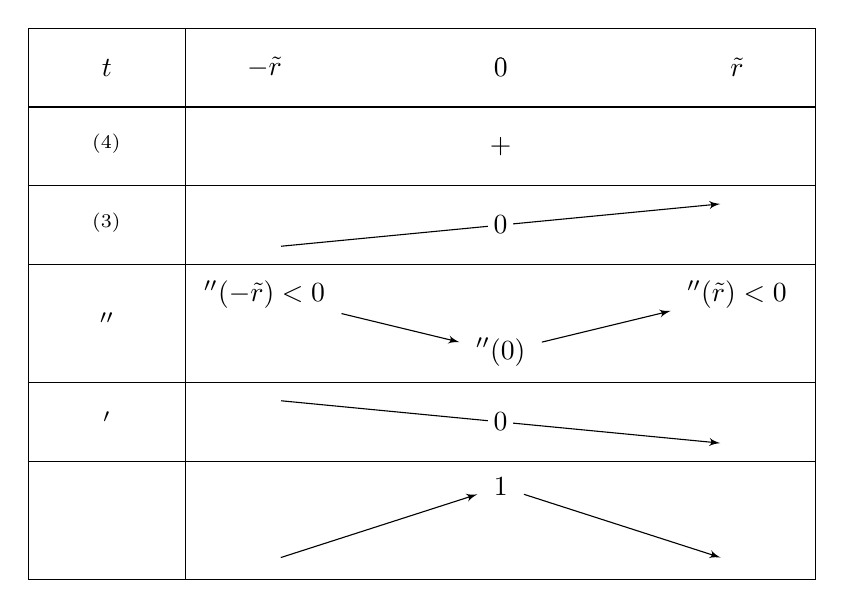
\begin{tikzpicture}
  \tkzTabInit[deltacl=1]{$t$ / 1,$\muc^{(4)}$ /1, $\muc^{(3)}$/1,$\muc''$ /1.5,$\muc'$ /1, $\muc$ /1.5 }{$-\tilde{r}$, $0$ , $\tilde{r}$}%
  \tkzTabLine{,,+,}
  \tkzTabVar{-/,R/$0$ ,+/}\tkzTabVal{1}{3}{0.5}{0}{0}
  \tkzTabVar{+/$\muc''(-\tilde{r})<0$,-/$\muc''(0)$ ,+/$\muc''(\tilde{r})<0$}
  \tkzTabVar{+/,R/$0$ ,-/}\tkzTabVal{1}{3}{0.5}{0}{0}
  \tkzTabVar{-/,+/1,-/}
\end{tikzpicture}
\end{center}
%%
\caption{Variations of $\muc$ and its derivatives. }\label{tab-var-mu}
\end{table}
%%%%%%%%%%%%%%%%%%%%%%%%%

Let us observe that the function $\theta : t \mapsto \muc(t)-\frac{t}{2} \muc'(t)$ is (strictly) decreasing in $[0,\tilde{r})$, since 
  \begin{align}
    \forall t\in (0,\tilde{r}),\    \theta'(t)=\frac{1}{2} \left(\muc'(t)-t\muc''(t) \right)=\frac{1}{2} \int_0^t\underbrace{(\muc''(u)-\muc''(t))}_{<0}du<0.
  \end{align}
  Hence, for all $k$ such that $k\stepsizen\in (0,\tilde{r})$, 
  \begin{align}
    \muc(k\stepsizen)-\frac{\stepsizen}{2} \muc'(k\stepsizen) &=\underbrace{\muc(k\stepsizen)-\frac{k\stepsizen}{2} \muc'(k\stepsizen)}_{=\theta(k\stepsizen)<\theta(0)=1} + \underbrace{\frac{(k-1)\stepsizen}{2} \muc'(k\stepsizen)}_{<0}<1.
  \end{align}

On the other hand, $\theta$ is (strictly) increasing on $(-\tilde{r}, 0]$ since 
  \begin{align}
    \forall t\in (-\tilde{r},0),\    \theta'(t)=\frac{1}{2} \left(\muc'(t)-t\muc''(t) \right)=\frac{1}{2} \int_0^t\underbrace{(\muc''(u)-\muc''(t))}_{<0}du>0.
  \end{align}
  As a consequence, for all $k$ such that $k\stepsizen\in (-\tilde{r},0)$, 
  \begin{align}
    \muc(k\stepsizen)+\frac{\stepsizen}{2} \muc'(k\stepsizen) &=\underbrace{\muc(k\stepsizen)-\frac{k\stepsizen}{2} \muc'(k\stepsizen)}_{=\theta(k\stepsizen)<\theta(0)=1} + \underbrace{\frac{(k+1)\stepsizen}{2} \muc'(k\stepsizen)}_{\leq 0}<1.
  \end{align}
  Thus we see that $\muc(k\stepsizen)+\frac{\stepsizen}{2} |\muc'(k\stepsizen)|<1$ for all $k\stepsizen \in(-\tilde{r},\tilde{r})\setminus\{0\}$, and we proceed similarly on all the intervals of the form $(x_{0,\nu}-r_\nu,x_{0,\nu}+r_\nu)$. By a compactness argument, there exists a constant $\beta<1$ such that $\muc(t)\leq \beta$ for all $t\in \TT\setminus \bigcup_{\nu=1}^N(x_{0,\nu}-r_{\nu},x_{0,\nu}+r_{\nu})$. For $n$ large enough, the inequality $\frac{\stepsizen}{2} \left(\sup_{t\in \TT} |\muc'(t)|\right)<1-\beta$ holds, and we see that $\muc(k\stepsizen) + \frac{\stepsizen}{2} |\muc'(k\stepsizen)|<1$ for all $t\in \TT\setminus \bigcup_{\nu=1}^N(x_{0,\nu}-r_{\nu},x_{0,\nu}+r_\nu)$.

  As a conclusion, we see that $\muc$ is a valid certificate for $(\veccontO,0)$ (see the optimality conditions of Proposition~\ref{prop-optim-cbp}), thus  $(\veccontO,0)$ is a solution of~\eqref{eq-thin-cbp}.  
\end{proof}

%%%%%%%%%%%%%%%%%%%%%%%%%%%%%%%%%%%%%%%%%%%
\subsection{Asymptotics of the Minimal Norm Certificates}

Observe that if the Twice Non-Degenerate Source Condition (Definition~\ref{defn-TNDSC}) holds, the hypotheses of Lemma~\ref{lem-source-cbp} are satisfied and $m_0$ is a solution to~\eqref{eq-thin-cbp} for $n$ large enough. In fact the associated minimal norm certificates (which thus exist) converge towards $\mut$.

\begin{prop}\label{prop-cv-cbpcertif}
  Let $m_0\in \Mm(\TT)$ satisfy the \textit{Twice Non-Degenerate Source Condition} (and $\mut$ the corresponding Third derivative (pre)certificate). Let $\qon$ be the minimal norm solution of~\eqref{eq-thin-dual-cbp}, and $\muon=\Phi^*\qon$. Then,
\begin{align}
    \lim_{n\to +\infty} \qon &=p_T \mbox{ for the $\Hh$ strong topology,}\\ 
    \lim_{n\to +\infty} \muon^{(k)} &=\mut^{(k)} \mbox{ in the sense of the uniform convergence, for all $k\in \NN$ up to the regularity of $\varphi$.} 
\end{align}
\end{prop}

\begin{proof}
  As mentioned above, the Twice Non-Degenerate Source Condition implies that Lemma~\ref{lem-source-cbp} applies to the function $\mut$, hence $\mut$ is a certificate for~\eqref{eq-thin-cbp}.
  As a result, $\|\qon \|\leq \|p_T\|$ and the sequence $(\qon )_{n\in\NN}$ is bounded in $\Hh$. We may extract a subsequence $p_{0,n'}$ which weakly converges towards some $\tilde{p}\in \Hh$, and then $\|\tilde{p}\|\leq \liminf_{n'\to +\infty}\|\qon \|\leq \|p_T\|$. Since $\Phi^*$ and $\Phi^{(k),*}$ are compact (see \cite[Lemma~1]{2016-duval-thinlasso}), we obtain that $\muc_{0,n'}^{(k)}=(\Phi^*p_{0,n'})^{(k)}$ converges toward $\tilde{\muc}^{(k)}\eqdef(\Phi^* \tilde{p})^{(k)}$ in the (strong) topology of uniform convergence. We immediately obtain that $\tilde{\muc}(t)\leq 1$ for all $t\in \TT$, and $\tilde{\muc}(x_{0,\nu})=1$, $\tilde{\muc}(x_{0,\nu})=0$ for all $\nu\in \{1,\ldots ,N \}$. 
  
  Moreover, applying Lemma~\ref{lem-cbp-dualspikes} to $\Phi^*\qon $ (observing that $x_\nu \in \Sright(r)\cap \Sleft(r)$), we get $\tilde{\muc}^{(3)}(x_{0,\nu})=0$. As a result, $\tilde{p}$ is admissible for~\eqref{eq-def-thirdderivcertif}, hence $\|p_T\|\leq \|\tilde{p}\|$. Thus in fact $\|p_T\|= \|\tilde{p}\|$ and $p_T=\tilde{p}$. Since the limit of the extracted subsequence does not depend on the choice of the subsequence, in fact the whole sequence converges. Moreover, the convergence is strong in $\Hh$ since $\lim_{n\to +\infty}\|\qon \|=\|p_T\|$. 
\end{proof}
As a consequence of the above convergence result, the third derivative precertificate controls the extended support on thin grids. 

\begin{prop}
  Let $m_0\in \Mm(\TT)$ (with $\{x_{0,1},\ldots x_{0,N}\}\subset \Gg_n$) such that the Twice Non Degenerate Source Condition holds.
  Then, for $n$ large enough, $m_0$ is a solution to~\eqref{eq-thin-cbp} and its extended support is given by:
  \begin{align}
    \extun (m_0)= \bigcup_{\nu=1}^N \Sright(r), \qandq  \extdn (m_0)= \bigcup_{\nu=1}^N \Sleft(r),
  \end{align}
  where
  \begin{itemize}
    \item $\Sright(r)$ is equal to $\{x_{0,\nu}\}$ or $\{x_{0,\nu}-\stepsizen,x_{0,\nu}\}$,
    \item $\Sleft(r)$ is  equal to $\{x_{0,\nu}\}$ or $\{x_{0,\nu},x_{0,\nu}+\stepsizen\}$.
  \end{itemize}   
  Moreover, one cannot have simultaneously $\Sright(r)=\{x_{0,\nu}-\stepsizen,x_{0,\nu}\}$ and $\Sleft(r)=\{x_{0,\nu},x_{0,\nu}+\stepsizen\}$.
  \label{prop-cbp-thin-extendedsup}
\end{prop}

\begin{proof}
By Lemma~\ref{lem-source-cbp}, $m_0$ is a solution to~\eqref{eq-thin-cbp} and $\mut$ is a solution to~\eqref{eq-thin-dual-cbp}. 
Applying Lemma~\ref{lem-cbp-dualspikes} to $\muon$, $\mut$, we see that $\Sright(r)$ is of the form $\emptyset$, $\{i\stepsizen\}$ or $\{(i-1)\stepsizen,i\stepsizen\}$, and that $\Sleft(r)$ is of the form $\emptyset$, $\{j\stepsizen\}$ or $\{j\stepsizen,(j+1)\stepsizen\}$, with $i\leq j$.
On the other hand, by the extremality relations between $\muon$ (solution of~\eqref{eq-thin-dual-cbp}) and $\mon$ (solution of~\eqref{eq-thin-cbp}), $x_{0,\nu}\in\Sright(r)$ and $x_{0,\nu}\in \Sleft(r)$. As a consequence $\Sright(r)$ is equal to $\{x_{0,\nu}\}$ or $\{x_{0,\nu}-\stepsizen,x_{0,\nu}\}$, and $\Sleft(r)$ is  equal to $\{x_{0,\nu}\}$ or $\{x_{0,\nu},x_{0,\nu}+\stepsizen\}$.

Now, since $\mut^{4}(0)\neq 0$, the fourth point of Lemma~\ref{lem-cbp-dualspikes} ensures that for $n$ large enough, one cannot have simultaneously $\Sright(r)=\{x_{0,\nu}-\stepsizen,x_{0,\nu}\}$ and $\Sleft(r)=\{x_{0,\nu},x_{0,\nu}+\stepsizen\}$.
\end{proof}

\begin{rem}
  As Proposition~\ref{prop-cbp-thin-extendedsup} shows, for each original spike, at most one pair of spikes appears at low noise: the original spike slightly shifted and either the immediate left neighbor shifted by $+\stepsizen/2$ or the immediate right neighbor shifted by $-\stepsizen/2$.
\end{rem}


%%%%%%%%%%%%%%%%%%%%%%%%%%%%%%%%%%%%%%%%%%%
\subsection{Proof of Theorem~\ref{thm-cbpasso-extended}}
\label{thm-cbpasso-extended-proof}

  We proceed by building a good candidate for $\muon$, making the ansatz that for all $\nu\in\{1,\ldots,N\}$, its saturation points satisfy
\begin{align}
  \mbox{if } \rho_\nu>0,& \mbox{ then }\Sright(r) = \{x_{0,\nu}-\stepsizen,x_{0,\nu}\}, \qandq \Sleft(r)=\{x_{0,\nu}\}, \\
  \mbox{if } \rho_\nu<0,& \mbox{ then }\Sleft(r) = \{x_{0,\nu}\}, \qandq \Sleft(r)=\{x_{0,\nu},x_{0,\nu}+\stepsizen\},
\end{align}
 and then, using Lemma~\ref{lem-mu0}, we prove that this candidate is indeed the minimal norm certificate.
 
To comply with the notations of Lemma~\ref{lem-mu0}, let us write  $\sum_{\nu=1}^N\alpha_{0,i}\delta_{x_{0,\nu}}= \sum_{k=0}^{\taillegridn-1} a_{0,k}\delta_{k\stepsizen}$, and $\Iup\eqdef \Idown\eqdef I\eqdef\enscond{i\in\seg{0}{\taillegridn-1}}{a_{0,i}\neq 0}$. 

For any choice of shift $(\epsilon_i)_{i\in I}\in \{-1,+1\}^{N}$, we set $\Jup \eqdef \Iup\cup\enscond{i+\varepsilon_i}{i\in I \qandq\varepsilon_i=-1}$ and $\Jdown\eqdef \Idown\cup\enscond{i+\varepsilon_i}{i\in I\qandq\varepsilon_i=+1}$.
  Since $|x_{0,\nu}-x_{0,\nu'}|> {2}{\stepsizen}$ for $\nu'\neq \nu$ and $n$ large enough, we have $\Card \Jup+\Card \Jdown=3\times \Card I=3N$. 
The idea is to find a choice of $\varepsilon$ such that $u_j > 0$ for all $j\in \Jup\setminus I$, and $v_j> 0$ for all $j\in \Jdown\setminus J$, where
\begin{align*}
  \begin{pmatrix} u_{\Jup}\\v_{\Jdown} \end{pmatrix}&\eqdef-(\Copt^*\Copt)^{-1}\begin{pmatrix}
    \bun_{\Jup}\\\bun_{\Jdown}\end{pmatrix}, \quad
\Copt \eqdef\begin{pmatrix}(\OpU+\frac{\stepsize}{2}\OpD)_{\Jup} &(\OpU-\frac{\stepsize}{2}\OpD)_{\Jdown}\end{pmatrix}\\
\OpU &\eqdef \Phi_{\Gg_n} \qandq \OpD\eqdef\Phi'_{\Gg_n}.
\end{align*} 


In this particular case where $\Iup= \Idown= I$, all $j$ in $(\Jup\setminus I)\cup (\Jdown\setminus I)$ may be uniquely written as $j=i+\varepsilon_i$ for some $i\in I$, where $\varepsilon_i\in\{-1,+1\}$.
We may swap the columns of $\Copt$ so as to reformulate the condition  $\begin{pmatrix} u_{\Jup}\\v_{\Jdown} \end{pmatrix}=-(\Copt^*\Copt)^{-1}\bun_{3N}$ into
\begin{align*}  
  \begin{pmatrix} \tilde{u}_I\\ \tilde{v}_I\\ \tilde{t}_I  \end{pmatrix}&=-(\Capt^*\Capt)^{-1}\begin{pmatrix}
    \bun_N\\\bun_N\ \\\bun_N 
  \end{pmatrix},
\end{align*}
where $\Capt \eqdef \begin{pmatrix} \OpU_I+ \frac{\stepsizen}{2}\OpD_I\diag(\varepsilon)  & \OpU_I-\frac{\stepsizen}{2}\OpD_I\diag(\varepsilon) & \OpU_{I+\varepsilon}-\frac{\stepsizen}{2}\OpD_{I+\varepsilon}\diag(\varepsilon)\end{pmatrix}$
and $\tilde{t}_i>0$ for all $i\in I$.
But a Taylor expansion yields
\begin{align*}
  \OpU_{I+\varepsilon}-\frac{\stepsizen}{2}\OpD_{I+\varepsilon}\diag(\varepsilon)&= \underbrace{\Phi_{x_0}}_{=\OpU_I}+ \frac{\stepsizen}{2}\underbrace{\Phi_{x_0}'\diag(\varepsilon)}_{=\OpD_I\diag(\varepsilon)}+ (\stepsizen)^3 \gamma_3\Phi^{(3)}_{x_0}\diag(\varepsilon)+o(\stepsizen^3),
\end{align*}
where we defined
\eql{\label{eq?defn-alphak}
	\gamma_k \eqdef \frac{1}{k!}- \frac{1}{(k-1)!\times 2}. 
}
Hence, we may apply Lemma~\ref{lem-apx-cbpdl} to $\Phi_{x_0}$, $\Phi_{x_0}'\diag(\varepsilon)$ and $\gamma_3\Phi^{(3)}_{x_0}\diag(\varepsilon)$ so as to obtain
\begin{align*}
  \tilde{t}_I &=  -\frac{1}{\gamma_3\stepsizen^3}\diag(\varepsilon) \rho +o\left(\frac{1}{\stepsizen^3}\right).
\end{align*}
Therefore it is sufficient to choose $\varepsilon = -\sign(\rho)$ to make all the components of $\tilde{t}_I$ nonnegative.

%  \left((\Phi_{x_0}^{(3)*}\projGam\Phi_{x_0}^{(3)})^{-1}\Phi_{x_0}^{(3)*}\Gamma_{x_0}(\Gamma_{x_0}^ \Gamma_{x_0})^{-1} 		\begin{pmatrix}      		\bun_{N}\\0    	\end{pmatrix}\right)

With that choice of $\varepsilon$, it remains to prove that
\eq{
	\max \left[\begin{pmatrix}(\OpU+\frac{\stepsize}{2}\OpD)_{\Jup^c}^* \\(\OpU-\frac{\stepsize}{2}\OpD)_{\Jdown^c}^* \end{pmatrix} \Copt \begin{pmatrix} u_{\Jup}\\v_{\Jdown} \end{pmatrix}\right]<1. 
}
Let us write $\tilde{p}_n\eqdef \Copt \begin{pmatrix} u_{\Jup}\\v_{\Jdown} \end{pmatrix}$. Since $\begin{pmatrix} u_{\Jup}\\v_{\Jdown} \end{pmatrix}=-(\Copt^*\Copt)^{-1}\bun_{3N}$, we get $\tilde{p}_n=\Copt^{+,*}\bun_{3N}$, and applying Lemma~\ref{lem-apx-cbpdl} to $\Phi_{x_0}$, $\Phi_{x_0}'\diag(\varepsilon)$ and $\gamma_3\Phi^{(3)}_{x_0}\diag(\varepsilon)$, we see that 
$\tilde{p}_n$ converges towards $p_T$ (using~\eqref{eq-qt-expression}).

By construction of $\tilde{p}_n$, 
\begin{align}
  &\forall j\in\Jup\setminus I, \ (\Phi^*\tilde{p}_n+\frac{\stepsizen}{2}(\Phi^*\tilde{p}_n)')(j\stepsizen)=1,\nonumber\\
  \qandq &\forall j\in\Jdown\setminus I, \  (\Phi^*\tilde{p}_n-\frac{\stepsizen}{2}(\Phi^*\tilde{p}_n)')(j\stepsizen)=1,\label{eq-cbp-pbaux}
  \intertext{which may be summarized as }
  &\forall i\in I, (\Phi^*\tilde{p}_n-\varepsilon_i\frac{\stepsizen}{2}(\Phi^*\tilde{p}_n)')((i+\varepsilon_i)\stepsizen)=1.\nonumber
   \end{align}

   Arguing as in the proof of point~\eqref{item-deriv4} in Lemma~\ref{lem-cbp-dualspikes} (replacing ``$1=\ldots$'' with ``$1\geq\ldots$'' and using that $\mut^{(4)}(x_{0,\nu})>0$), we may prove that for $n$ large enough, $(\Phi^*\tilde{p}_n+\varepsilon_i\frac{\stepsizen}{2}(\Phi^*\tilde{p}_n)')((i-\varepsilon_i)\stepsizen)<1$.

   Then, by the same argument of compactness and local concavity as in point~\eqref{item-deriv2} of Lemma~\ref{lem-cbp-dualspikes}, we observe that 
   \begin{align*}
  \enscond{k\in \seg{0}{\taillegridn-1}}{(\Phi^*\tilde{p}_n+\frac{\stepsizen}{2}(\Phi^*\tilde{p}_n)')(k\stepsizen)\geq 1}\subset \Jup,\\
 \enscond{k\in \seg{0}{\taillegridn-1}}{(\Phi^*\tilde{p}_n-\frac{\stepsizen}{2}(\Phi^*\tilde{p}_n)')(k\stepsizen)\geq 1}\subset \Jdown,
\end{align*}
and those inclusions are in fact equalities.
That precisely means that $\max \left[\begin{pmatrix}(\OpU+\frac{\stepsize}{2}\OpD)_{\Jup^c}^* \\(\OpU-\frac{\stepsize}{2}\OpD)_{\Jdown^c}^* \end{pmatrix}\tilde{p}_n\right]<1$.

Hence, by Lemma~\ref{lem-mu0}, $\Phi^*\tilde{p}_n$ is the minimal norm certificate $\muon$ and $(\Jup\stepsizen,\Jdown\stepsizen)$ is the extended support. This concludes the proof.
% \end{proof}



%%%%%%%%%%%%%%%%%%%%%%%%%%%%%%%%%%%%%%%%%%%
\subsection{Proof of Corollary~\ref{cor-cbp-extended}}
\label{prop-asympto-constant-cbp-proof}


The result is a consequence of~Theorem~\ref{thm-abstract-cbp} with the extended support provided by Theorem~\ref{thm-cbpasso-extended}. With the notations of~\cite[Appendix C.2]{2016-duval-thinlasso}, the constants are given by
\begin{align*}
  C^{(1)}_n\eqdef\left(\frac{c_{1,n}c_{5,n}}{c_{4,n}}+c_{2,n} \right)^{-1}\qandq
  C^{(2)}_n\eqdef \min\left(c_{3,n},\frac{c_{5,n}}{c_{4,n}}\right) .
\end{align*}
Replacing the constants $c_1,\ldots, c_3$
%of the proof of Theorem~\ref{thm-abstract-cbp} (see~\ref{sec-continuous-abstract-proofs} and~\cite[Appendix C.2]{2016-duval-thinlasso})
with the expressions corresponding to the continuous framework, and using Lemma~\ref{lem-apx-cbpdl} we get
\begin{align}\label{eq-cbp-cst-asympt-1}
	c_{1,n}&= \norm{R_{\Iup\cup\Idown}\Copt^+}  
	\sim 
	\frac{1}{(\stepsizen)^3}\normb{\begin{pmatrix}
    (\Phi_{x_0}^{(3),*}\projGam \Phi_{x_0}^{(3)})^{-1}\Phi_{x_0}^{(3),*}\projGam \\
    0
  \end{pmatrix}}_{\infty,\Hh}\\
  	\label{eq-cbp-cst-asympt-2}
  	c_{2,n}&= 
	\normb{\begin{pmatrix} \tilde{u}_I\\\tilde{v}_I \end{pmatrix}}
	\sim 
	\frac{1}{(\stepsizen)^3} 
	\normb{
		\begin{pmatrix}\rho \\ 0 \end{pmatrix}
	}_{\infty}\\
	\label{eq-cbp-cst-asympt-3}
  	c_{3,n} &= 
  	\left(\norm{R_{(\Jup\setminus\Iup)\cup(\Jdown\setminus\Idown)}\Copt^+}_{\infty,\Hh}\right)^{-1}
	\left(\min_{i\in I}\tilde{t}_i\right)
		\sim 
		\frac{
			\min_i \left| \frac{1}{\gamma_3} \rho_i \right|  
		}{
			\norm{(\Phi_{x_0}^{(3),*}\projGam \Phi_{x_0}^{(3)})^{-1}\Phi_{x_0}^{(3),*}\projGam}_{\infty,\Hh}
		}
\end{align}
where $\gamma_k$ is defined in~\eqref{eq?defn-alphak}.

As for $c_{4,n}$ and $c_{5_n}$, the expressions given in~\cite[Appendix C.2]{2016-duval-thinlasso} yield a pessimistic bound for the low noise regime, and we are led to make finer majorizations.
  Using the reformulation~\eqref{eq-reparam-cbpasso} of the C-BP as a (positive) \lasso, we have to ensure that $p_{\la}\eqdef \frac{1}{\la}( y- \OpU\veccont -\OpD\shiftcont
  )$ satisfies   
\begin{align*}
    \max \left[  \begin{pmatrix}
(\OpU^*+\frac{\stepsizen}{2} \OpD^*)_{(\Jup)^c}\\ (\OpU^*-\frac{\stepsizen}{2} \OpD^*)_{(\Jdown)^c}
  \end{pmatrix}p_{\la}
%  \begin{pmatrix}
%    y- \OpU\veccont -\OpD\shiftcont
%\end{pmatrix}
\right]<1
\end{align*}
where $\OpU \eqdef \Phi_{\Gg_n}$, $\OpD\eqdef\Phi'_{\Gg_n}$. 
  Let $\Copt \eqdef\begin{pmatrix}(\OpU+\frac{\stepsize}{2}\OpD)_{\Jup} &(\OpU-\frac{\stepsize}{2}\OpD)_{\Jdown}\end{pmatrix}$, $\projGam$ be the orthogonal projector onto $\ker \Copt^*=(\Im \Copt)^\perp$, and $\omega\eqdef \Phi^*\projGam w$. Since 
  \eq{
  	y - \OpU\veccont -\OpD\shiftcont= w- \Copt(\Copt^*\Copt)^{-1}\Copt^*w + \la \Copt(\Copt^*\Copt)^{-1}\bun_{3N} = \projGam w  +\la \Copt^{+,*}\bun_{3N}, 
	}
	we are led to check that
  \begin{align}
    (\omega +\la \muon)(j\stepsizen) + \frac{\stepsizen}{2} (\omega +\la \muon)'(j\stepsizen) &<\la \quad \mbox{ for all } j\in (\Jup)^C,\label{eq-tight-snr-cbpU}\\
    (\omega +\la \muon)(j\stepsizen) - \frac{\stepsizen}{2} (\omega -\la \muon)'(j\stepsizen) &<\la \quad \mbox{ for all } j\in (\Jdown)^C\label{eq-tight-snr-cbpD},
  \end{align}
  where $\muon\eqdef \Phi^*(\Copt^*\Copt)^{-1})\bun_{3N}$ yields the minimal norm certificate 
  \eq{
  	\begin{pmatrix}
    (\muon  +\frac{\stepsizen}{2}\muon)(\Gg_n)\\  (\muon  -\frac{\stepsizen}{2}\muon)(\Gg_n) 
  \end{pmatrix}=\begin{pmatrix}(\OpU+\frac{\stepsize}{2}\OpD)^* \\(\OpU-\frac{\stepsize}{2}\OpD)^*\end{pmatrix}(\Copt^*\Copt)^{-1}\bun_{3N}.
  }

Given $0<r<\frac{1}{2}\min_{\nu\neq \nu'}|x_{0,\nu}-x_{0,\nu'}|$, let $N(r)\eqdef\bigcup_{\nu}(x_{0,\nu}-r,x_{0,\nu}+r)$ be a neighborhood of the $x_{0,\nu}$'s. By the Twice Non-Degenerate Source condition, we may choose $r>0$, such that
\begin{align*}
  -\tilde{k}_1\eqdef \sup_{t\in N(r)}\mut''(t)< 0,\qandq  \tilde{k}_{2}\eqdef \inf_{t\in N(r)}\mut^{(4)}(t)>0.
\end{align*}
By compactness, $\tilde{k}_3\eqdef \sup_{t\in\TT\setminus N(r)}\mut(t)<1$.

Let us recall that $\muon\to \mut$ in the sense of the uniform convergence (and similarly for the derivatives). As a result, for $n\in\NN$ large enough, 
\eql{
  	\sup_{t\in N(r)}(\muon)''(t)<-\frac{\tilde{k}_1}{2}<0,
	\:  
	\inf_{t\in N(r)}(\muon)^{(4)}(t)>\frac{\tilde{k}_{2}}{2}>0, 
	\: 
  	\sup_{t\in\TT\setminus N(r)} \muon(t) <\frac{1+\tilde{k}_3}{2}<1, \label{eq-cbp-const-muO}
}
\eq{
  	\frac{\stepsizen}{2} \norm{(\muon)^{(3)}}_{\infty} \leq \frac{\tilde{k}_1}{8},
	\qandq 
	\frac{\stepsizen}{2} \norm{(\muon)'}_{\infty} \leq \frac{1-\tilde{k}_3}{6}.
}
Now, we assume that $\frac{\normH{w}}{\la}$ is small enough, so that 
\begin{align*}
  \norm{(\Phi^{(k)})^*}_{\infty,\Hh}\frac{\normH{w}}{\la} <\frac{\tilde{k}_1}{8}, 
  \mbox{ for } k\in\{2,3\}, \quad  
  \norm{(\Phi^{(4)})^*}_{\infty,\Hh}\frac{\normH{w}}{\la} <\frac{\tilde{k}_2}{4},
\end{align*}
\begin{align}
	\qandq  \norm{(\Phi^{(k)})^*}_{\infty,\Hh}\frac{\normH{w}}{\la} <\frac{1-\tilde{k}_3}{6}, 
	\mbox{ for } k\in\{0,1\},\label{eq-cbp-const-noise}
\end{align}

Then, using the fact that and $|\omega^{(k)}|(t)\leq \norm{(\Phi^{(k)})^*}_{\infty,\Hh}\normH{w}$ and  $\stepsizen\leq 1$, we obtain
\begin{align*}
  \sup_{t\in \TT\setminus N(r)} \left(\frac{\omega}{\la} + \muon + \frac{\stepsizen}{2}\left|(\frac{\omega}{\la} + \muon)'\right|\right)(t)<1.
\end{align*}
Thus it remains to prove that for each $\nu\in\{1,\ldots, N\}$, 
\begin{align}
  \left(\frac{\omega}{\la} + \muon + \frac{\stepsizen}{2}(\frac{\omega}{\la} + \muon)'\right)(t)<1 \mbox{ for } t \in (x_{0,\nu}-r,x_{0,\nu}+r)\setminus \Sright(r),\label{eq-cbp-const-sat1}\\
\qandq \left(\frac{\omega}{\la} + \muon - \frac{\stepsizen}{2}(\frac{\omega}{\la} + \muon)'\right)(t)<1 \mbox{ for } t \in (x_{0,\nu}-r,x_{0,\nu}+r)\setminus \Sleft(r)\label{eq-cbp-const-sat2}.
\end{align} 
We only deal with the case  $\Sright(r)=\{x_{0,\nu} \}$, $\Sleft(r)=\{x_{0,\nu},x_{0,\nu}+\stepsizen\}$, the symmetric case being similar. 
Let $f\eqdef \frac{1}{\la}\omega(\cdot-x_{0,\nu})+\muon(\cdot-x_{0,\nu})$. By definition of $\projGam$, $\omega(x_{0,\nu})=\omega'(x_{0,\nu})=\omega(x_{0,\nu}+\stepsizen)-\frac{\stepsizen}{2}\omega(x_{0,\nu}+\stepsizen)=0$, so that
\eql{\label{eq-cbp-const-fval}
f(0)=1, \quad f'(0)=1, \qandq f(\stepsizen)-\frac{\stepsizen}{2}f'(\stepsizen)=1.
}
Moreover, from Eq.~\eqref{eq-cbp-const-muO} to~\eqref{eq-cbp-const-noise}, and letting $k_1=\frac{\tilde{k}_1}{8}$, $k_2=\frac{\tilde{k}_2}{4}$, we deduce that 
\eql{\label{eq-cbp-const-fsec}
 \forall t\in(-r,r),\quad f''(t)+\frac{\stepsize}{2}|f^{(3)}(t)| <-k_1<0, \qandq f^{(4)}(t)>k_2>0,
}
so that the strict concavity of $f-\frac{\stepsizen}{2} f'$ implies that $(f-\frac{\stepsizen}{2} f')(t)<1$ for $t\in (-r,-\stepsizen)\cup (0,r)$.

It remains to prove that  $(f+\frac{\stepsizen}{2} f')(t)<1$ for $t\in (-r,r)\setminus (-\stepsizen,0]$. A Taylor expansion of $f$ and $f'$ yields (writing as usual $\gamma_k=\frac{1}{k!}- \frac{1}{(k-1)!\times 2}$)
\begin{align*}
  \underbrace{1-(f(\stepsize)- \frac{\stepsizen}{2}f(\stepsizen))}_{=0} &= \underbrace{1- f(0)- \frac{\stepsizen}{2}f'(0)}_{=0} -\stepsizen^3\gamma_3 f^{(3)}(0) - \stepsizen^4\gamma_4f^{(4)}(0) +R_1(\stepsizen),\\
  1-(f(-\stepsizen)+\frac{\stepsizen}{2} f'(-\stepsizen))&=  \underbrace{1- f(0)+ \frac{\stepsizen}{2}f'(0)}_{=0} +\stepsizen^3\gamma_3 f^{(3)}(0) - \stepsizen^4\gamma_4f^{(4)}(0) + R_2(\stepsizen).
\end{align*}
Adding both equations we get 
\begin{align}
  1-(f(-\stepsizen)+\frac{\stepsizen}{2} f'(-\stepsizen))&= -2\stepsizen^4\gamma_4f^{(4)}(0)+ (R_1+R_2)(\stepsizen)\\ % -\stepsize^5\int_0^1 (f^{(5)}(s\stepsize)-f^{(5)}(-s\stepsize))\left(\frac{(1-s)^4}{4!} -\frac{(1-s)^3}{2\times 3!}\right) \d s.
  \label{eq-minoration-dl} &\geq 2(-\gamma_4) k_2\stepsizen^4 + (R_1+R_2)(\stepsizen), 
\end{align}
where
\begin{align}R_1+R_2(h) = \stepsizen^5\int_0^1 (-f^{(5)}(s\stepsizen)+f^{(5)}(-s\stepsizen))\left(\frac{(1-s)^4}{4!} -\frac{(1-s)^3}{2\times 3!}\right) \d s,\label{eq-rest-integral}
\end{align}
\begin{align}  
	\mbox{with} \quad \norm{f^{(5)}}_{\infty} \leq \norm{\frac{1}{\la}\omega^{(5)}}_\infty+\norm{(\muon)^{(5)}}_\infty=O(1).
\end{align}
Hence, 
\begin{align}
  1-(f(-\stepsizen)+\frac{\stepsizen}{2} f'(-\stepsizen))&\geq \underbrace{2(-\gamma_4) k_2}_{>0}\stepsizen^4 + O(\stepsizen^5)>0.
\end{align}
Moreover,by the strict concavity of $f+\frac{\stepsizen}{2} f'$, we also deduce that $(f+\frac{\stepsizen}{2} f')(t)<1$ for $t\in (-r,-\stepsizen]\cup (0,r)$, thus we get the local inequalities~\eqref{eq-cbp-const-sat1} and~\eqref{eq-cbp-const-sat2}, hence the global inequalities~\eqref{eq-tight-snr-cbpU} and~\eqref{eq-tight-snr-cbpD}.

To conclude, the constants in the condition on $\frac{\normH{w}}{\la}$ are $O(1)$, and gathering the asympotics for $c_{1,n},c_{2,n},c_{3,n}$ we obtain $C^{(1)}_{n}=O(\stepsizen^3)$, $C^{(2)}_n= O(1)$.
% \end{proof}

Eventually, the proof of~\eqref{eq-lipsch-cbp} follows from~\eqref{eq-cbp-cst-asympt-1} and~\eqref{eq-cbp-cst-asympt-2}. 




%%%
%\bibliographystyle{plain}
%\bibliography{bibliography}
\printbibliography


\end{document}

